\documentclass{beamer}
\usepackage[utf8]{inputenc}
\usetheme{Berlin}
\usecolortheme{whale}
\useoutertheme{infolines}
\useinnertheme{rectangles}

\title[]{Microservicios y su relación con la calidad del software}
\author[M. Rey, U. Ramirez]{Martín Rey; Ulises Ramirez}
\date[JCS UNaM 2019]{Instituto de Desarrollo, Innovación e Investigación en Informática \\ FCEQyN - UNaM \\ 2019}

\setbeamertemplate{navigation symbols}{}

\usepackage{graphicx}
\usepackage{soul}
\usepackage{hyperref}
\begin{document}

\frame{\titlepage}

\begin{frame}
    \frametitle{Agenda}
    \tableofcontents
\end{frame}

\section{Quiénes somos?}

\begin{frame}
    \frametitle{About us}
	\begin{block}{Martín Rey}
Docente - Investigador - Desarrollador \\
\textbf{Temas de interés:} Ciencia de Datos, Agilidad, Auditoría.
  	\end{block}

	\begin{block}{Ulises Ramirez}
Alumno - Investigador - Desarrollador \\
\textbf{Temas de interés:} Procesamiento de Lenguaje Natural, Inteligencia Artificial, computo distribuido y paralelo
  	\end{block}

\end{frame}

\section{Introducción}

\begin{frame}
	\frametitle{Una definición extremadamente simple}
	Es una aplicación que hace \textbf{un conjunto de operaciones} y las hace \textbf{muy bien}. \\
	Utilizando un ejemplo \emph{de otro mundo}, proponemos un viaje en el tiempo...\\
\end{frame}

\begin{frame}
	\frametitle{PitStop de F1 en 1950}
	\begin{figure}[htp]
	\centering
	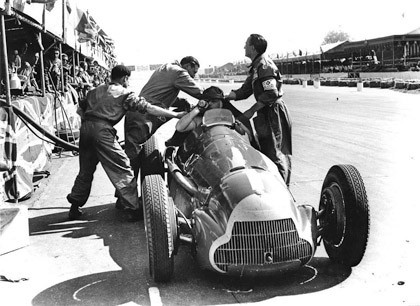
\includegraphics[scale=0.4]{img/f1-antes.jpeg}
	\end{figure}

	Pocos mecanicos, capaces de hacer cualquier operación. \\
	Mucho tiempo, y poca escalabilidad dadas las características del personal.
\end{frame}

\begin{frame}
	\frametitle{PitStop de F1 en 2019}
	\begin{figure}[htp]
	\centering
	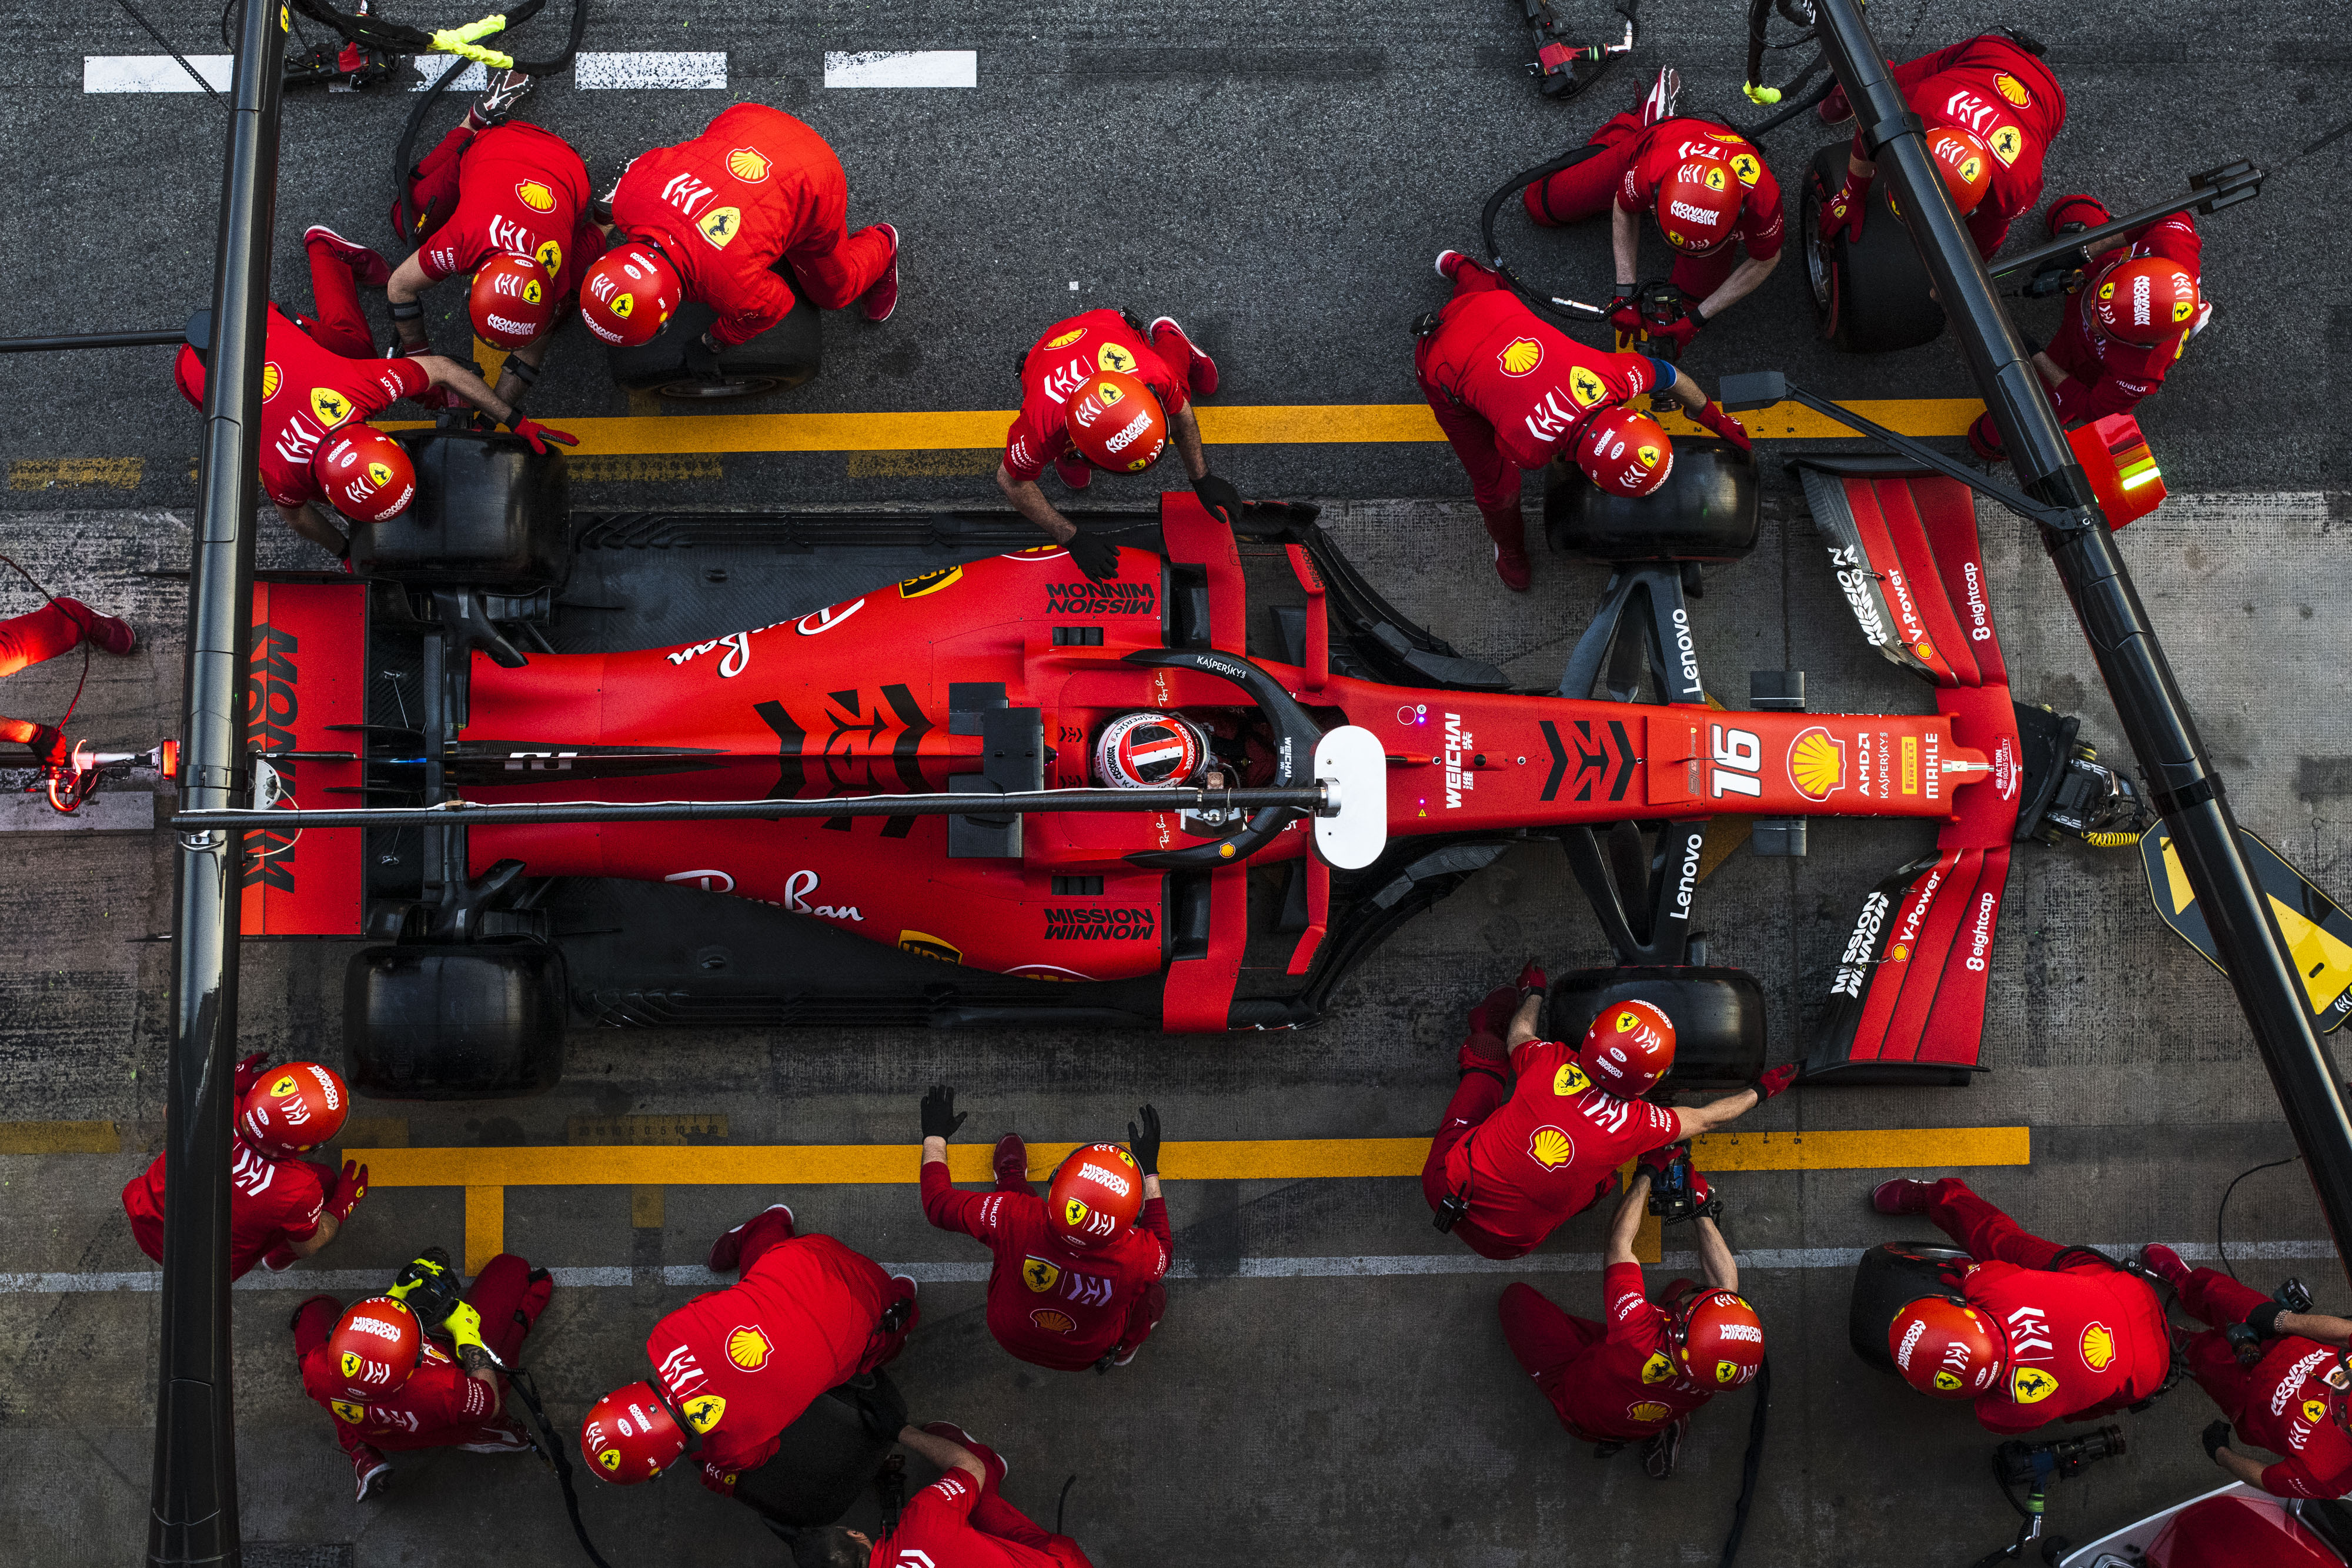
\includegraphics[scale=0.25]{img/f1-ahora.jpeg}
	\end{figure}

	Muchos mecanicos, muy especializados hacen una cosa y muy bien. \\
	Poco tiempo (-2 segs), y menor complejidad en la tarea de cada persona.
\end{frame}

\begin{frame}
    \frametitle{Un poco de análisis}
    \begin{itemize}
    	\item \textbf{Especialización}: una persona que sabe sacar la rueda, una persona que sabe colocarla y una persona que sabe como manejar la herramienta para desajustar/ajustar.
		\item \textbf{Escalabilidad}: un auto tiene N ruedas, se multiplican por N las personas del punto anterior.
		\item \textbf{Complejidad}: ¿se ve incrementada? A simple vista, sí. Hay muchas personas trabajando, pero en términos de las tareas individuales, es mucho más simple.
    \end{itemize}
\end{frame}

\begin{frame}
    \frametitle{Pero acá vinimos a hablar de software (?)}
	En una \textbf{arquitectura} de microservicios, una persona del caso anterior es un \textbf{servicio}. \\
	Un servicio es software que realiza un conjunto de tareas lógicamente relacionadas y se mantiene \emph{relativamente} aislado de los demás. \\
	Esta tarea podría ser: enviar una notificación, calcular el sueldo a cobrar de un empleado, agregar un filtro a una foto, grabar un audio, etc.
\end{frame}

\begin{frame}
    \frametitle{Pero acá vinimos a hablar de software (?) II}
	De esta manera, los servicios que responden a un requerimiento se pueden \textbf{escalar} en forma individual. Además de que, ante un cambio o error, \textbf{solo los servicios afectados se modifican} y pasan por el flujo de CI + CD, no toda la aplicación.
\end{frame}

\begin{frame}
    \frametitle{Una definición larga, de uno que sabe de esto}
	"\textsl{In short, the microservice architectural style is an approach to developing a \textbf{single application as a suite of small services}, each running in its own process and \textbf{communicating with lightweight mechanisms}, often an HTTP resource API. These services are built around business capabilities and independently deployable by fully automated deployment machinery. There is a bare minimum of \textbf{centralized management} of these services, which may be written in \textbf{different programming languages and use different data storage technologies}. }" \href{https://martinfowler.com/articles/microservices.html}{Martin Fowler}.
\end{frame}

\begin{frame}
	\frametitle{Comparación con el enfoque monolítico}
	\begin{figure}[htp]
	\centering
	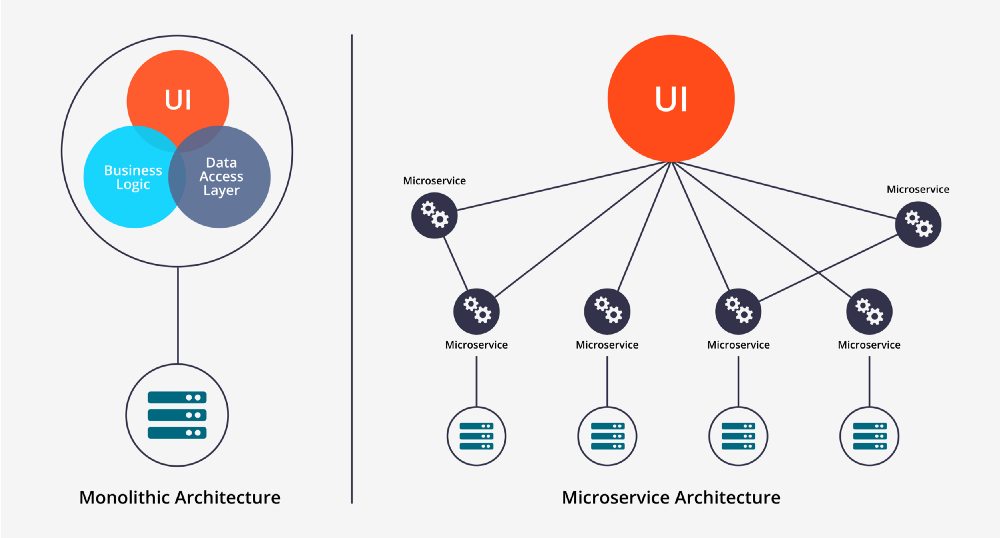
\includegraphics[scale=0.33]{img/comparacion.png}
	\end{figure}
\end{frame}


\begin{frame}
    \frametitle{Comparación con el enfoque monolítico}
	\begin{block}{Monolítico}
	\begin{itemize}
		\item Una aplicación tiene su UI, base de datos y código del backend donde se define la lógica del negocio del problema a resolver.
		\item Los cambios que se requiera hacer implican una actualización de todo el backend.
		\item Existen relaciones lógicas entre los componentes del backend definidas sobre los elementos que provee la herramienta utilizada en el desarrollo (módulos, clases, etc).
		\item La escalabilidad implica la replicación de toda la aplicación en diferentes instancias y contar con un balanceador de carga. Pudiendo hacer algo similar con la base de datos.
	\end{itemize}
  	\end{block}
\end{frame}

\begin{frame}
	\frametitle{Comparación con el enfoque monolítico}
	\begin{block}{Microservicios}
	\begin{itemize}
		\item Cada componente de una aplicación puede ser implementada como un servicio.
		\item Ante un cambio o corrección de errores se pueden aplicar cuestiones como feature flags, sobre un servicio en particular para que solo su funcionalidad se actualice.
		\item Cada servicio puede ser implementado de la manera que la tecnología que se determine utilizar recomiende para el caso.
		\item La escalabilidad se puede realizar un servicio a la vez.
	\end{itemize}
  	\end{block}
\end{frame}

\begin{frame}
	\frametitle{Ejemplo}
	\begin{figure}[htp]
	\centering
	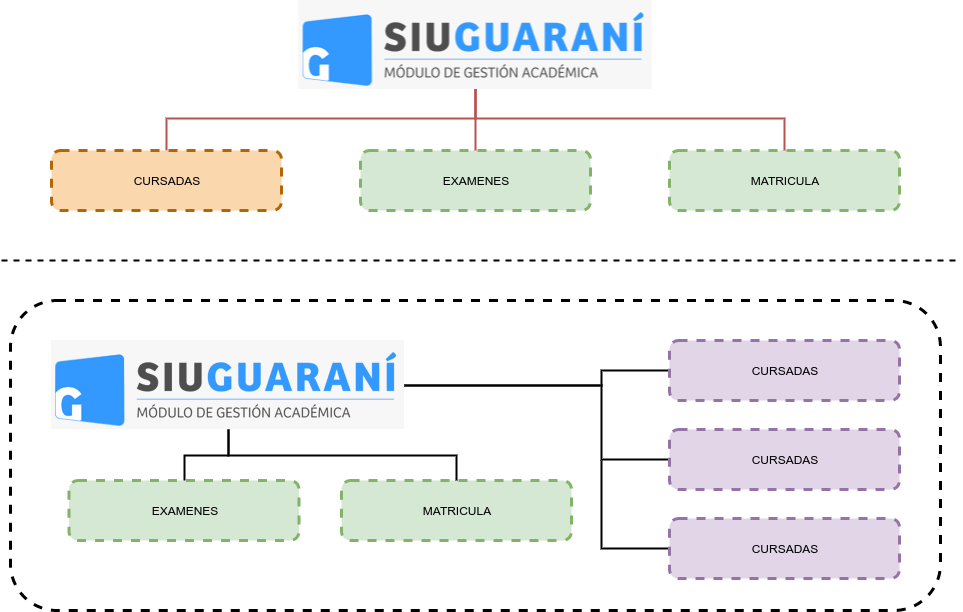
\includegraphics[width=0.95\linewidth]{img/ejemplo-guarani.png}
	\end{figure}
\end{frame}

\begin{frame}
	\frametitle{Algo sobre orquestación}
	\begin{figure}[htp]
	\centering
	
\includegraphics[width=0.95\linewidth]{img/orquestacion_1.png}
	\end{figure}
\end{frame}

\begin{frame}
  \frametitle{Algo sobre orquestación (2)}
	\begin{figure}[htp]
	\centering
	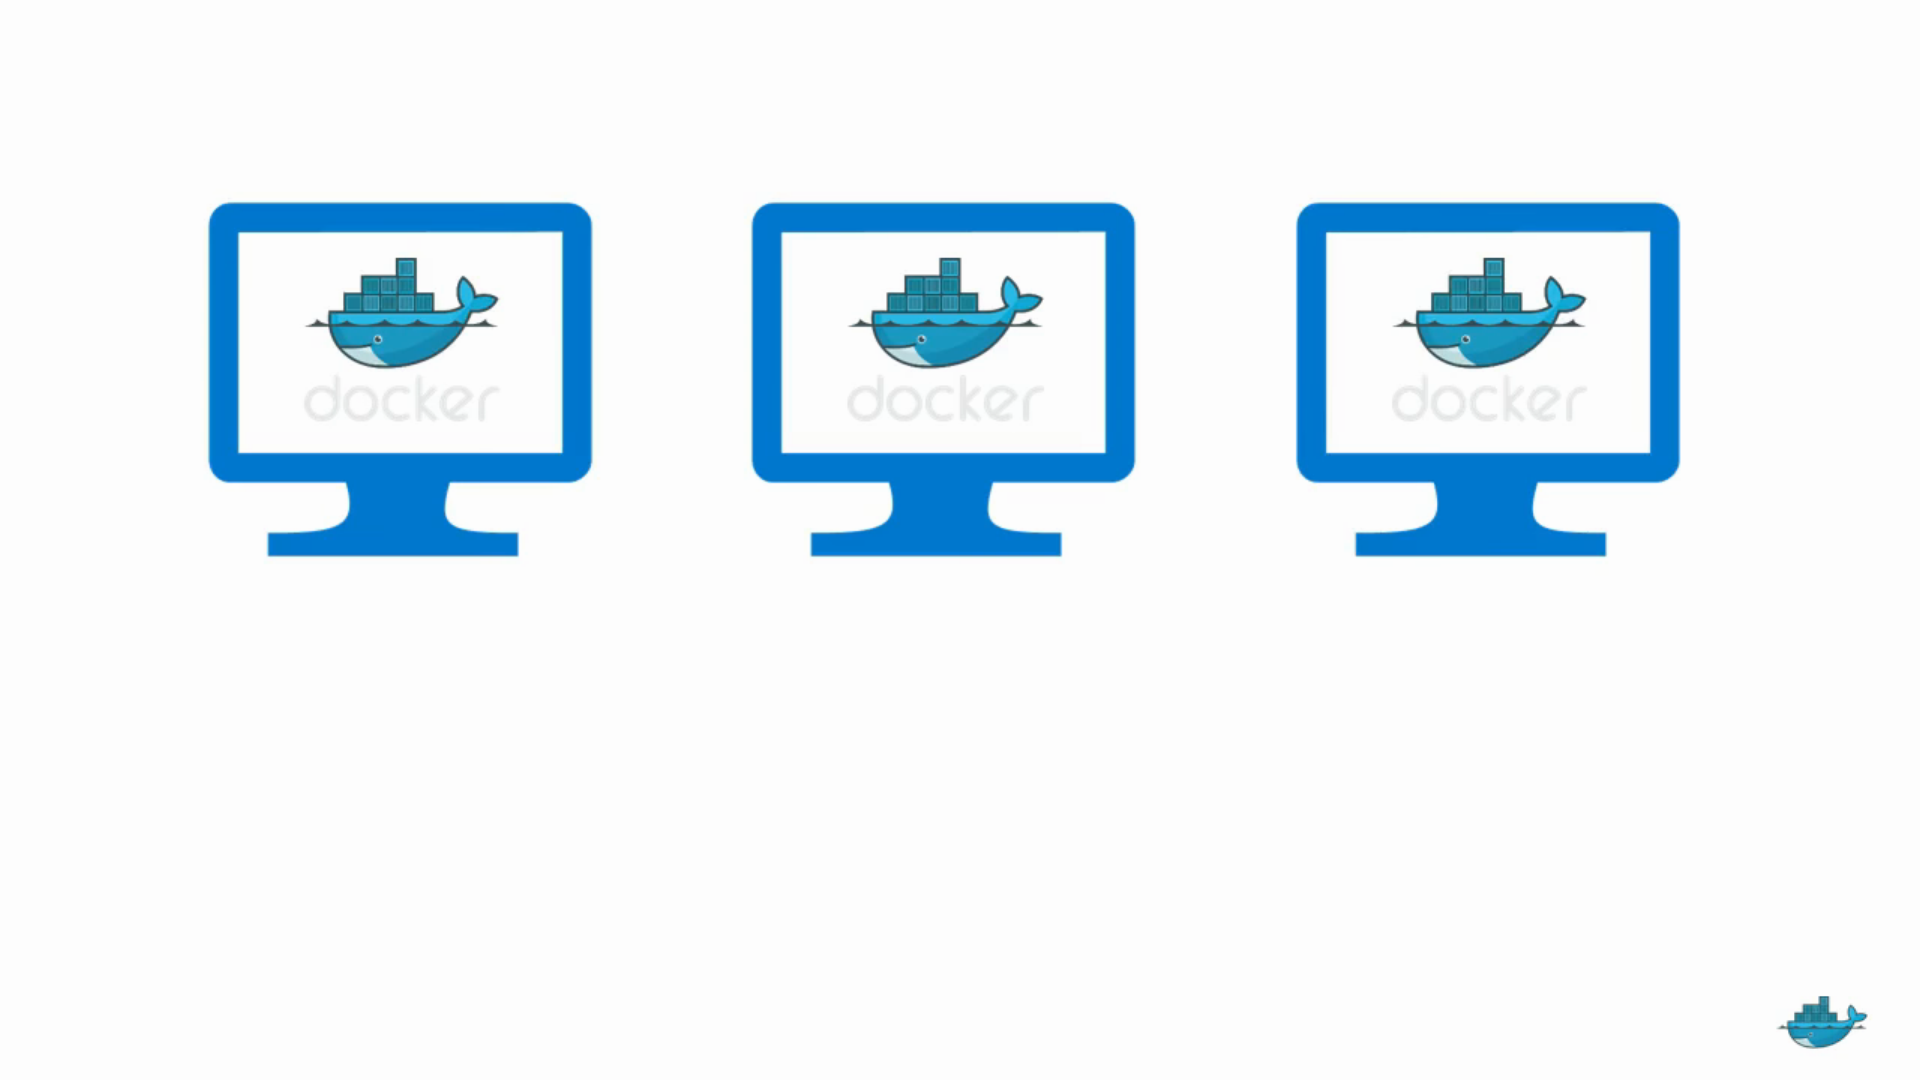
\includegraphics[width=0.95\linewidth]{img/orquestacion_2.png}
	\end{figure}
\end{frame}


\begin{frame}
  \frametitle{Algo sobre orquestación (3)}
	\begin{figure}[htp]
	\centering
	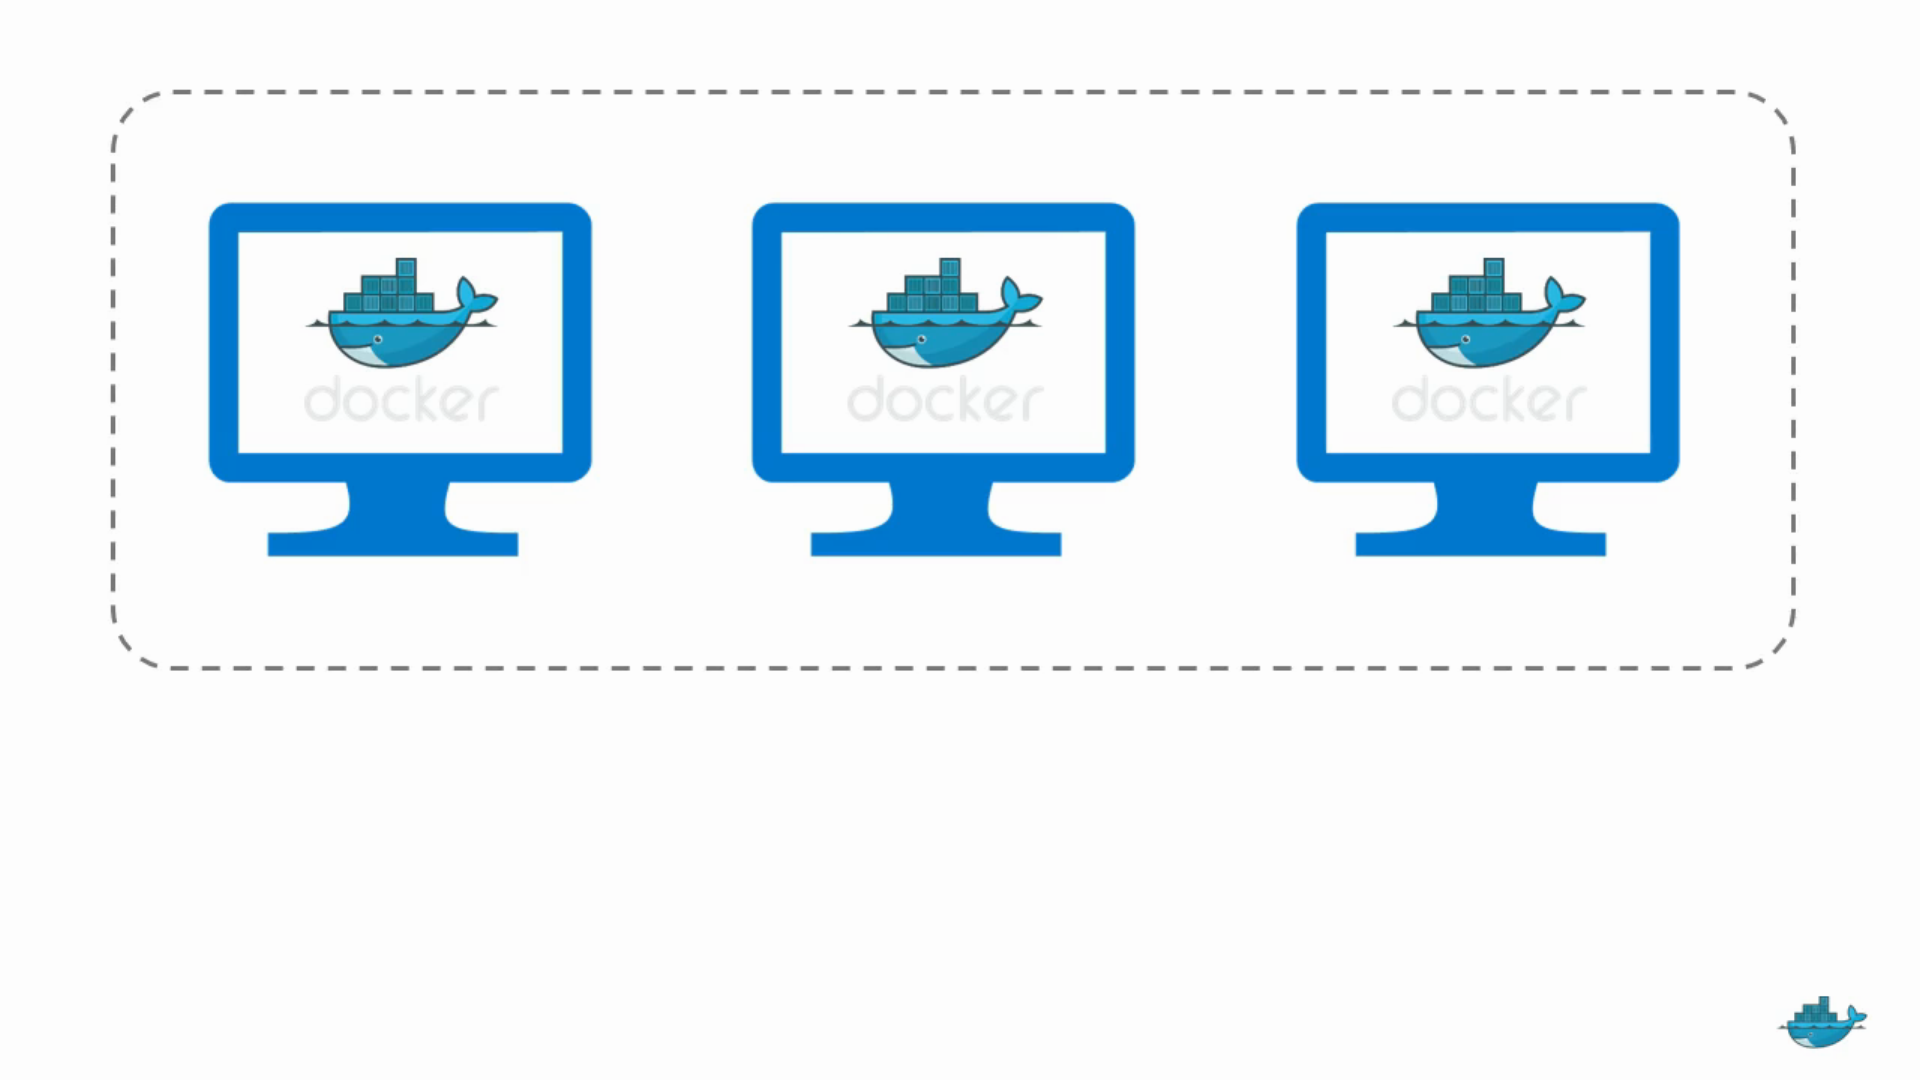
\includegraphics[width=0.95\linewidth]{img/orquestacion_3.png}
	\end{figure}
\end{frame}

\begin{frame}
  \frametitle{Algo sobre orquestación (4)}
	\begin{figure}[htp]
	\centering
	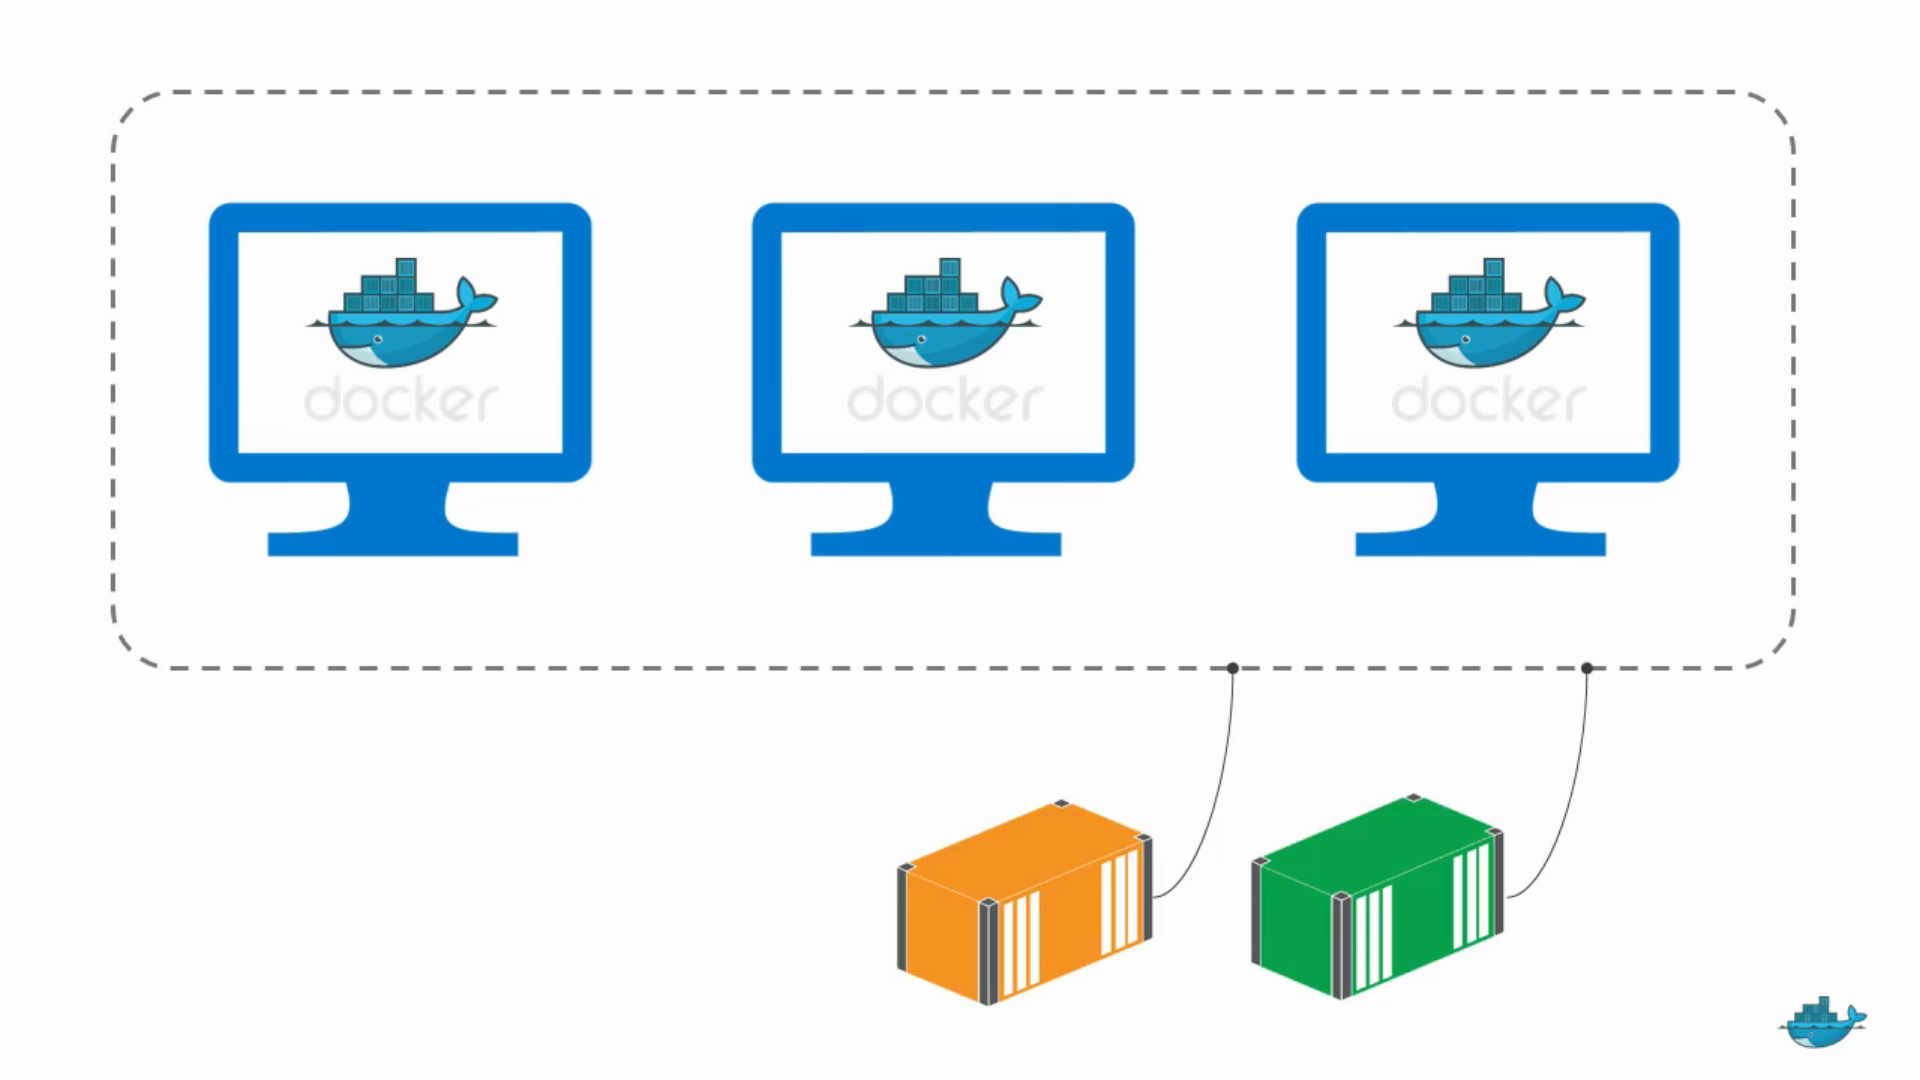
\includegraphics[width=0.95\linewidth]{img/orquestacion_4.png}
	\end{figure}
\end{frame}

\begin{frame}
  \frametitle{Algo sobre orquestación (5)}
	\begin{figure}[htp]
	\centering
	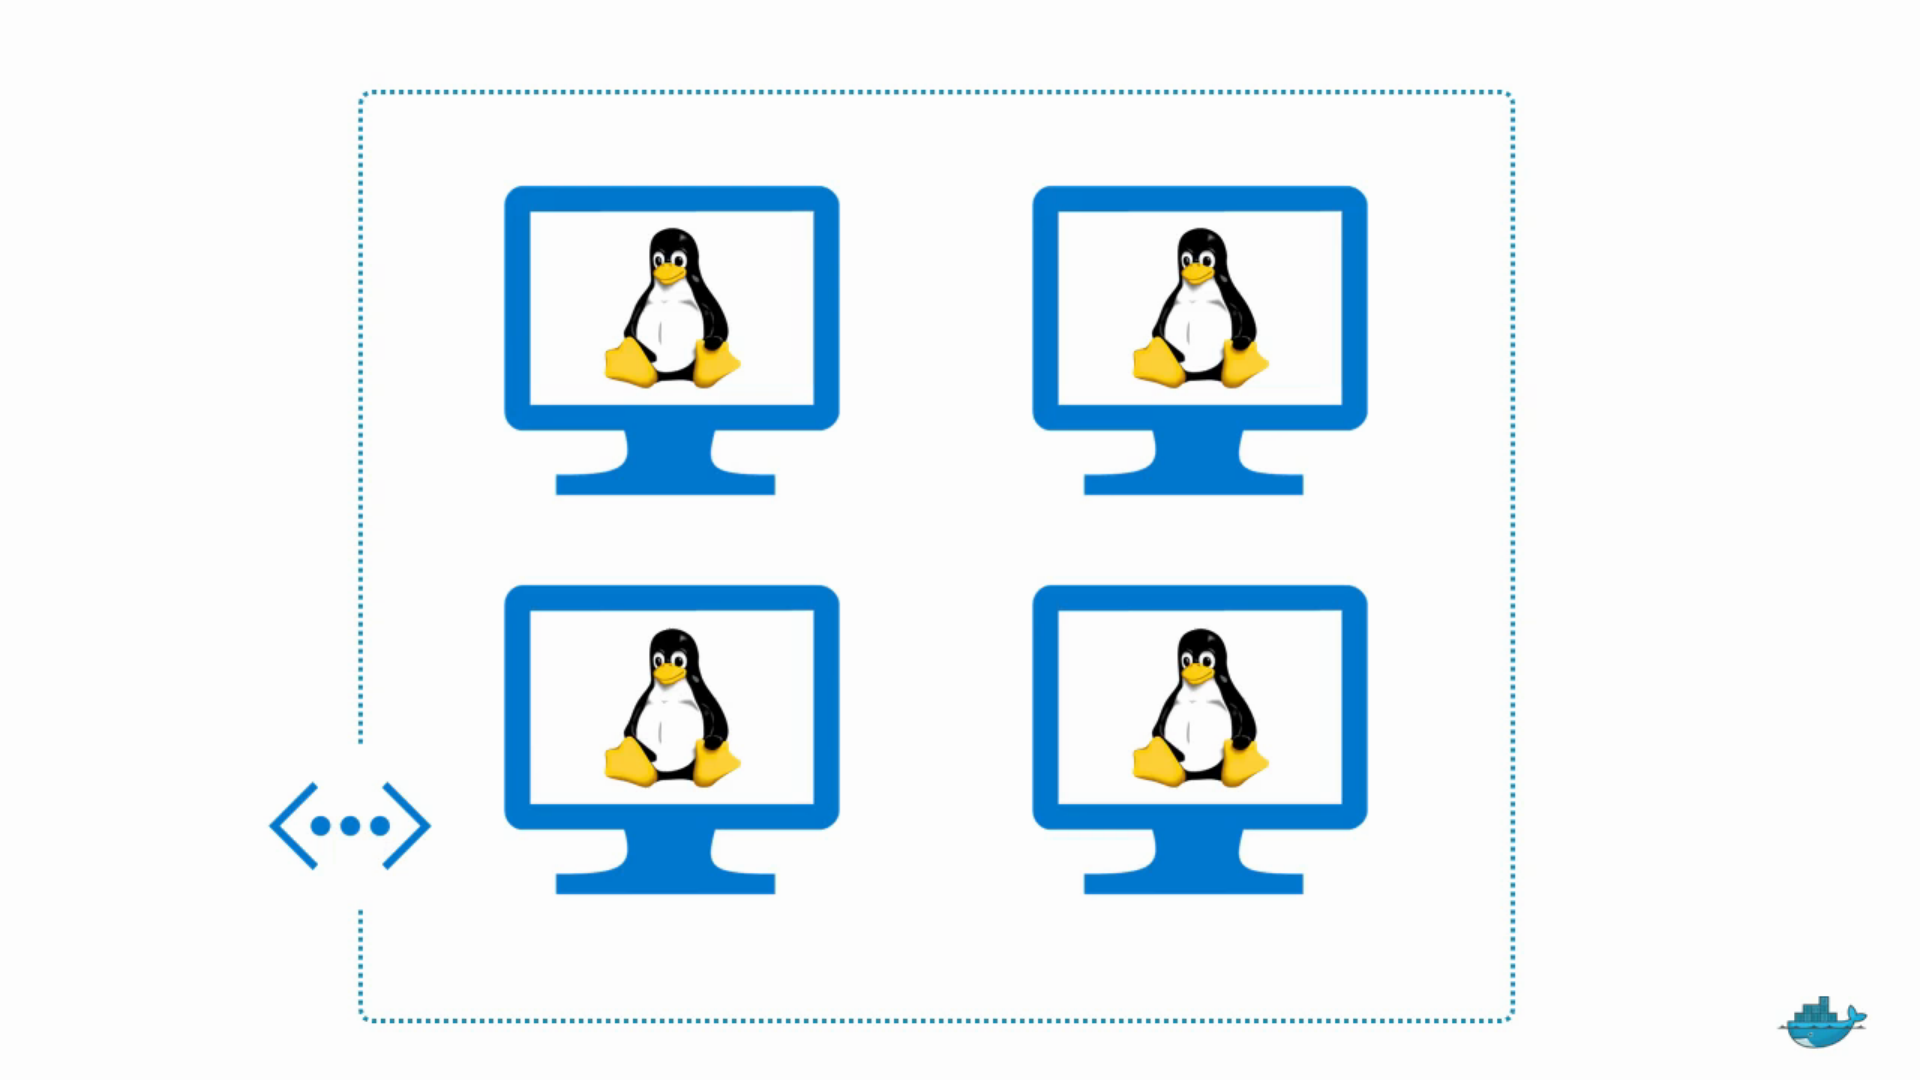
\includegraphics[width=0.95\linewidth]{img/orquestacion_5.png}
	\end{figure}
\end{frame}

\begin{frame}
  \frametitle{Algo sobre orquestación (6)}
	\begin{figure}[htp]
	\centering
	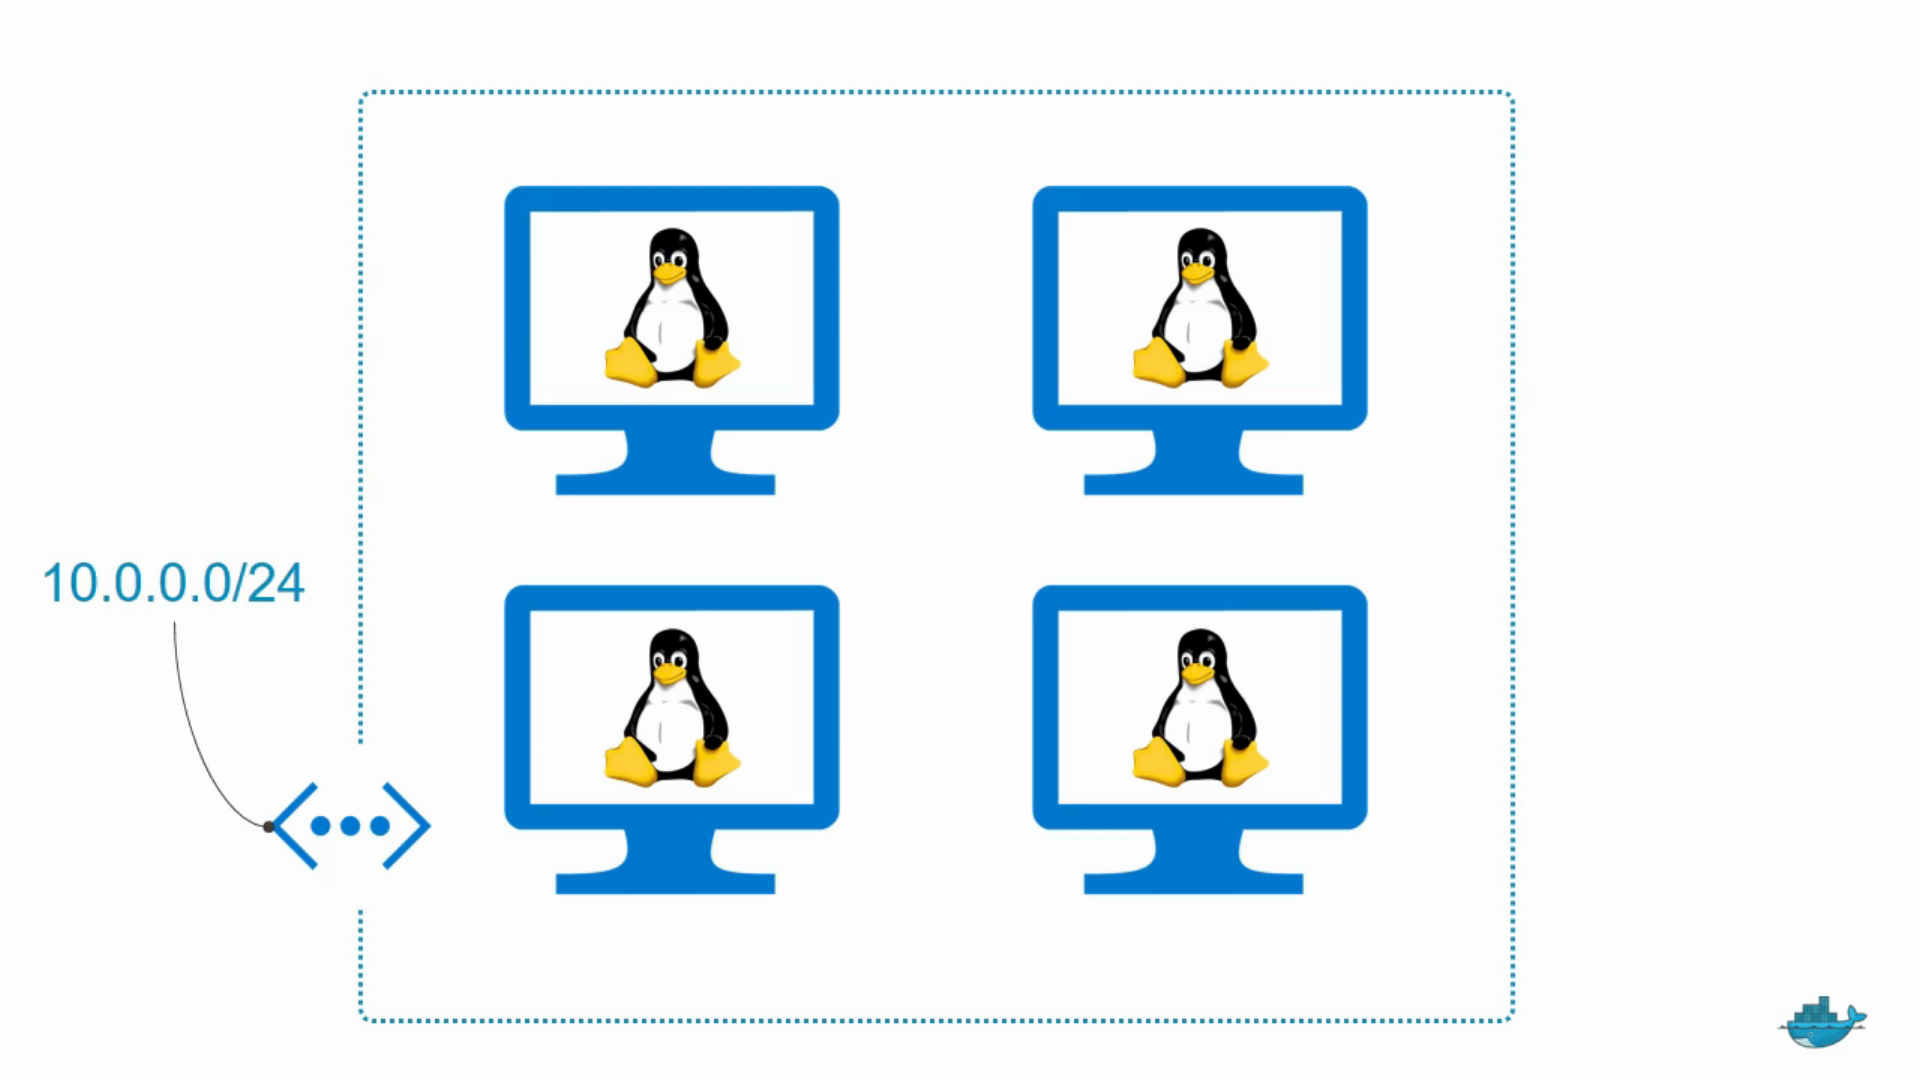
\includegraphics[width=0.95\linewidth]{img/orquestacion_6.png}
	\end{figure}
\end{frame}

\begin{frame}
  \frametitle{Algo sobre orquestación (7)}
	\begin{figure}[htp]
	\centering
	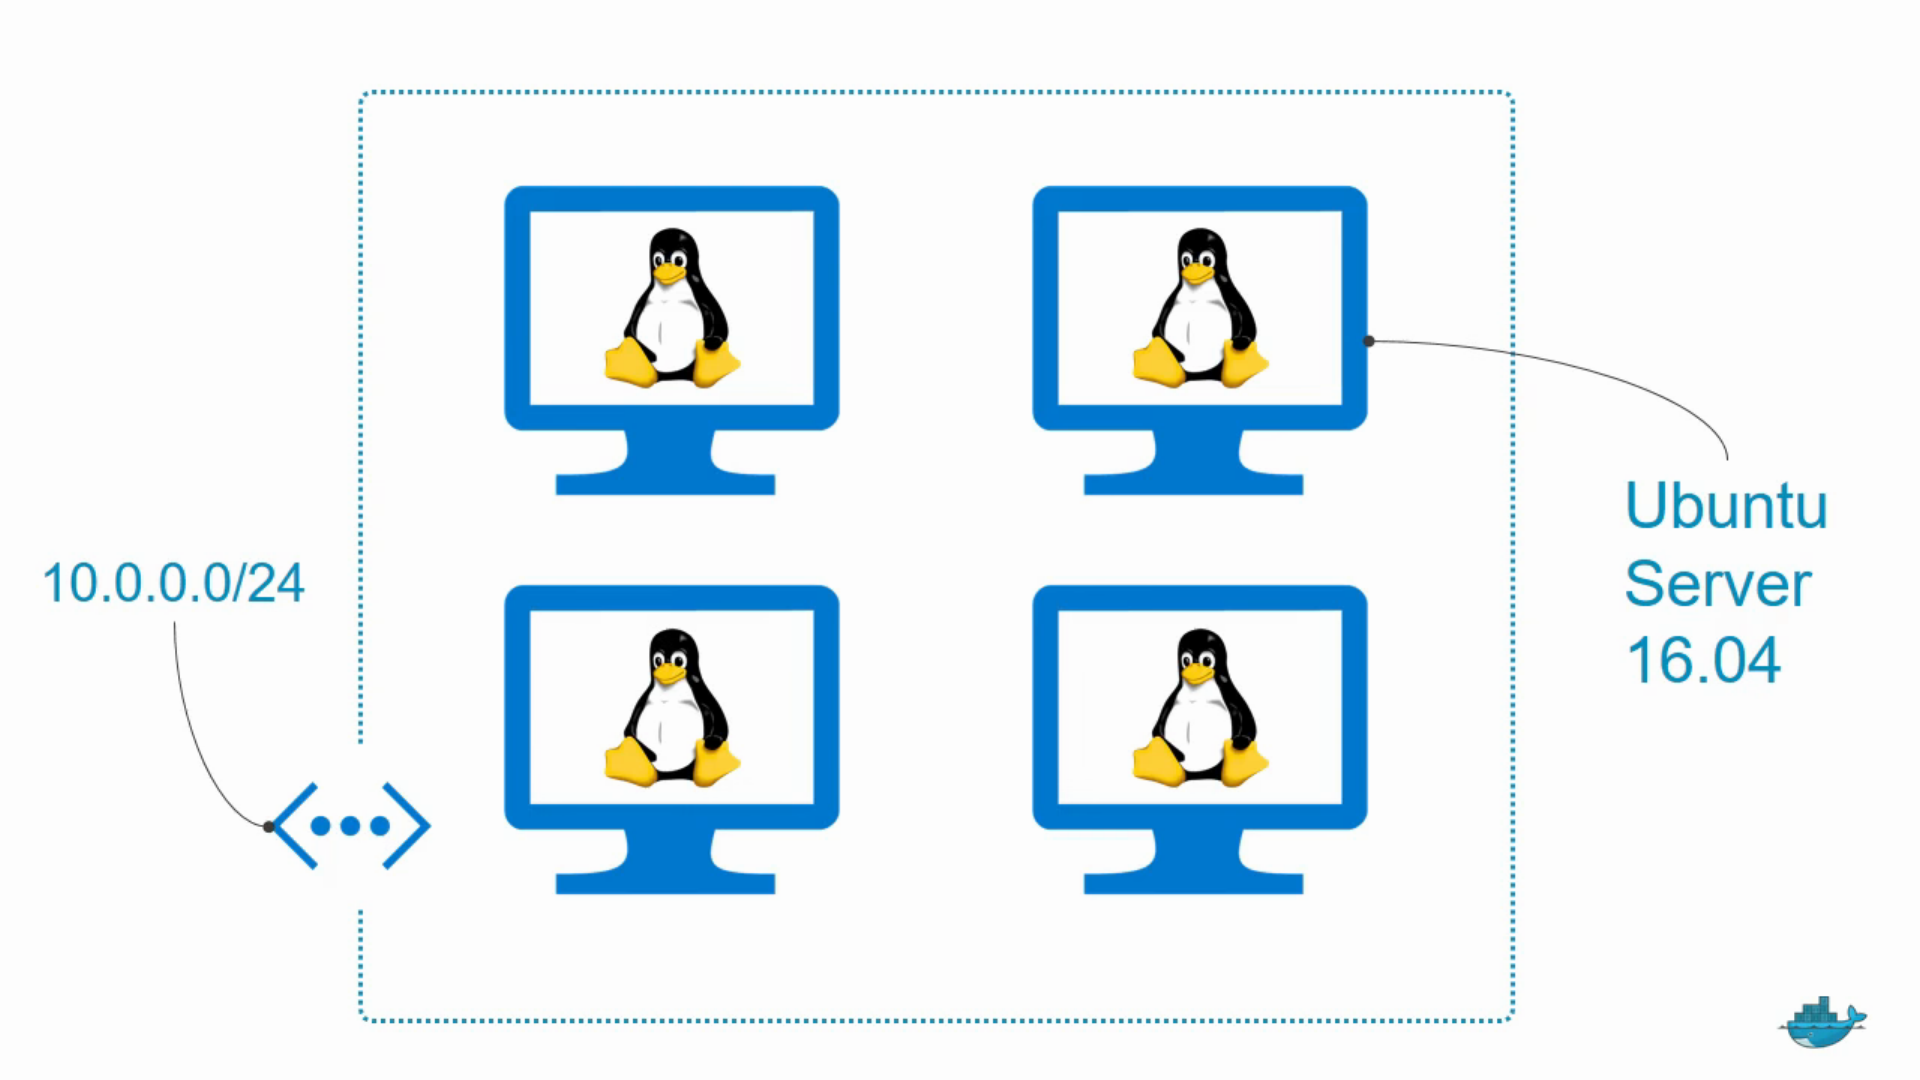
\includegraphics[width=0.95\linewidth]{img/orquestacion_7.png}
	\end{figure}
\end{frame}
\begin{frame}
  \frametitle{Algo sobre orquestación (8)}
	\begin{figure}[htp]
	\centering
	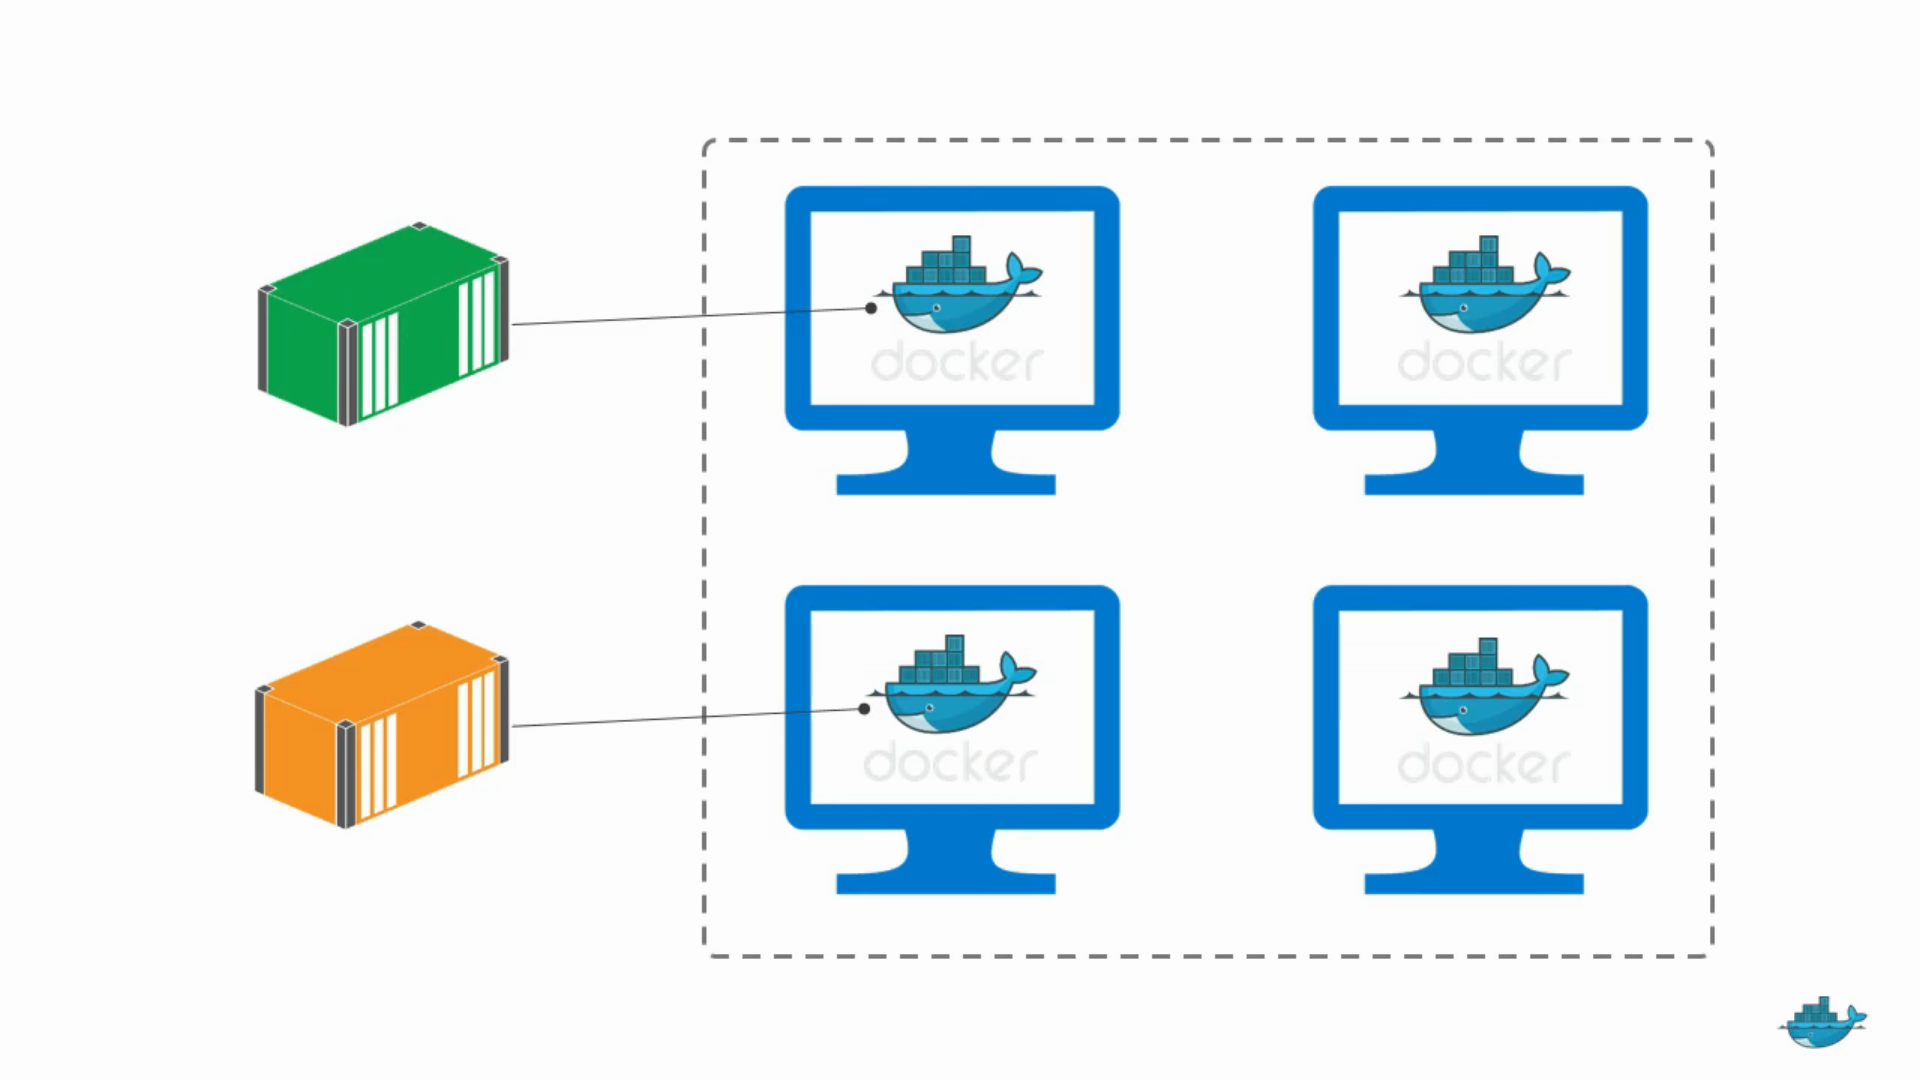
\includegraphics[scale=]{img/orquestacion_8.png}
	\end{figure}
\end{frame}

\begin{frame}
  \frametitle{Algo sobre orquestación (9)}
	\begin{figure}[htp]
	\centering
	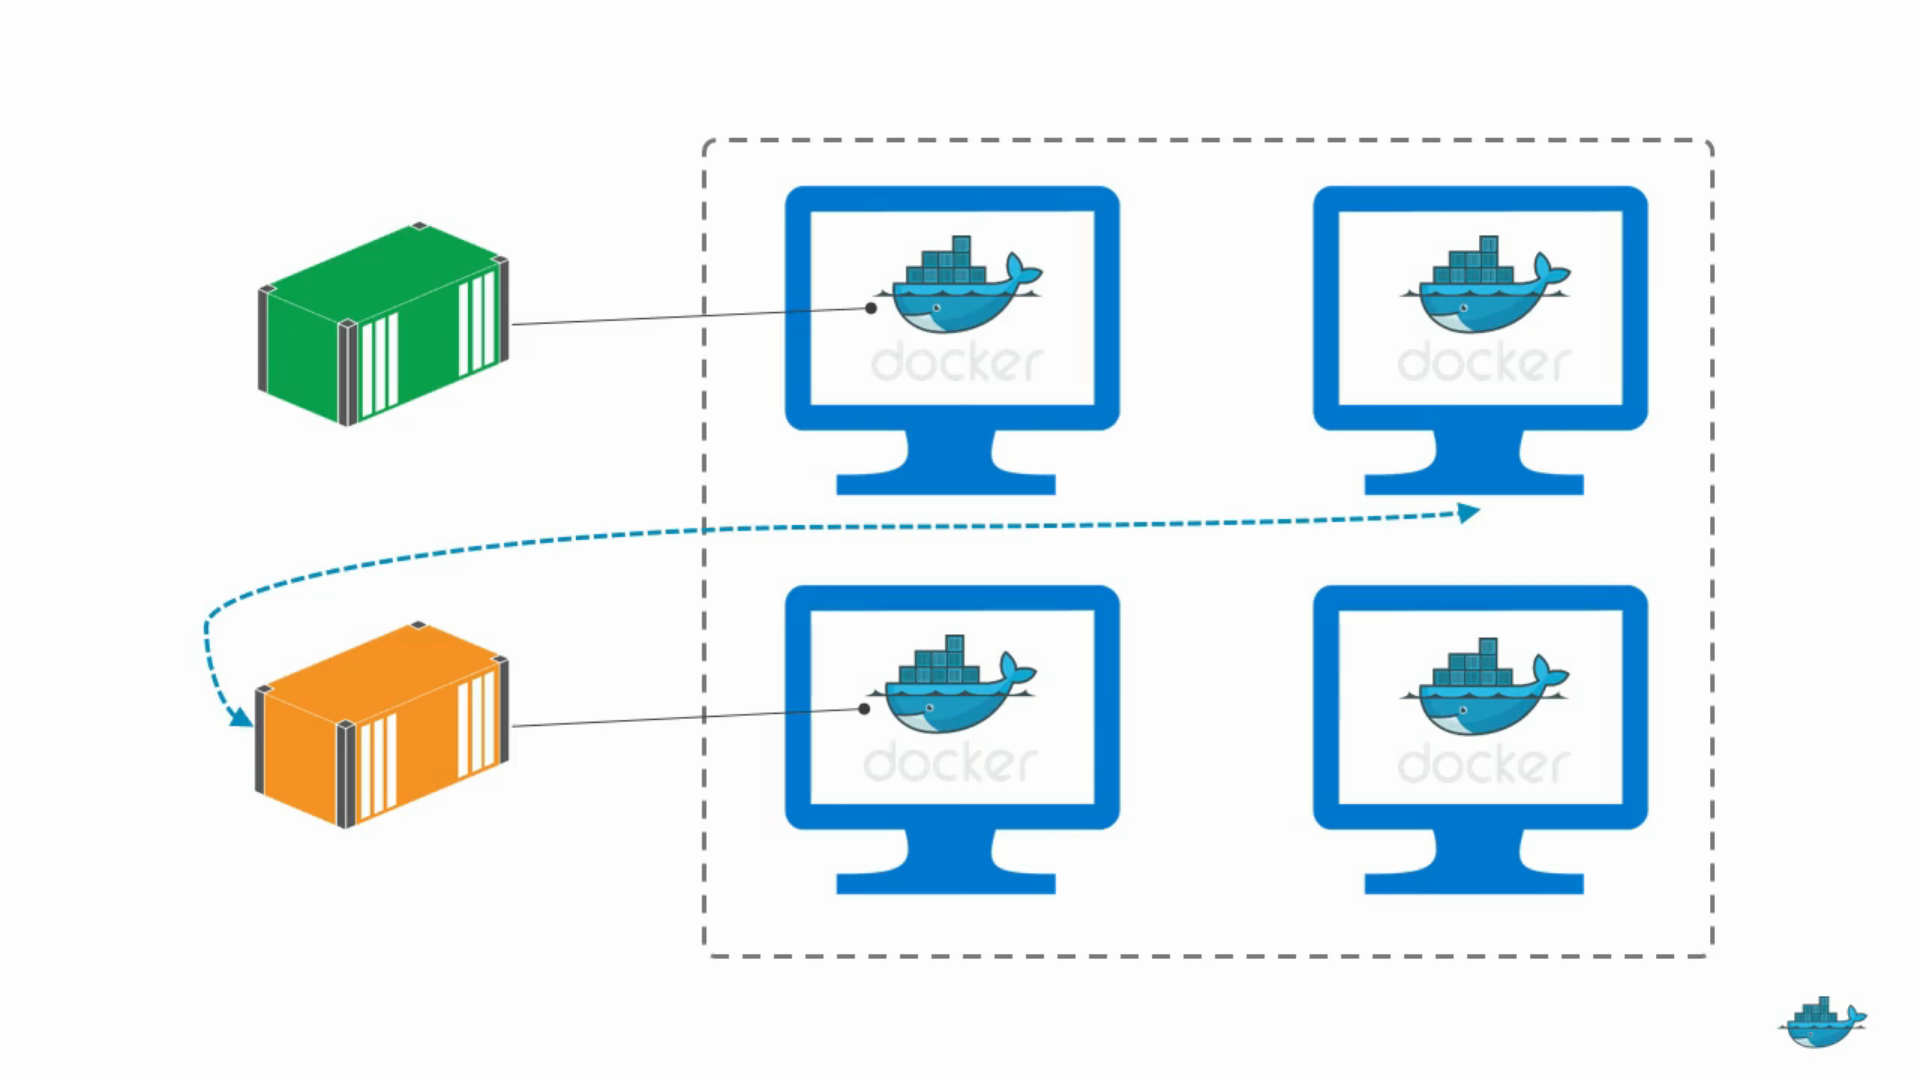
\includegraphics[width=0.95\linewidth]{img/orquestacion_9.png}
	\end{figure}
\end{frame}

\begin{frame}
  \frametitle{Algo sobre orquestación (10)}
	\begin{figure}[htp]
	\centering
	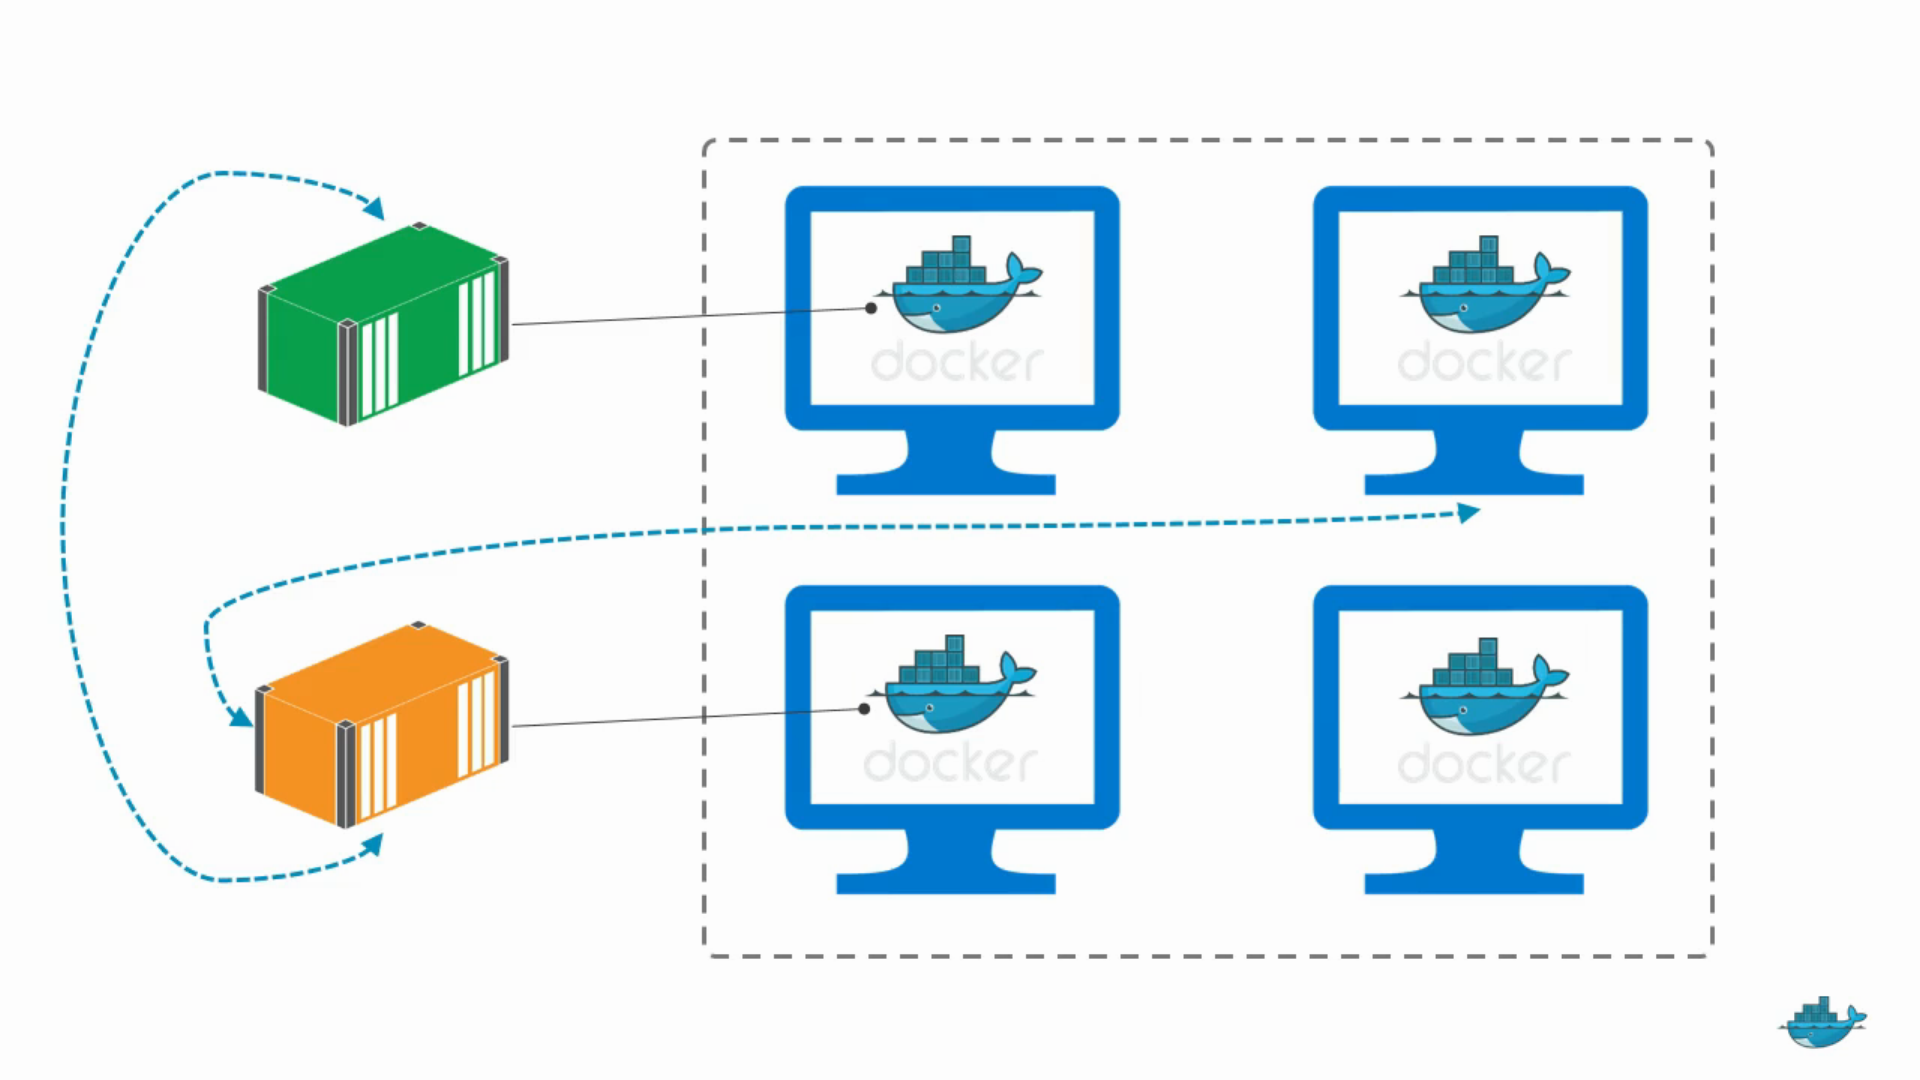
\includegraphics[width=0.95\linewidth]{img/orquestacion_10.png}
	\end{figure}
\end{frame}

\begin{frame}
  \frametitle{Algo sobre orquestación (11)}
	\begin{figure}[htp]
	\centering
	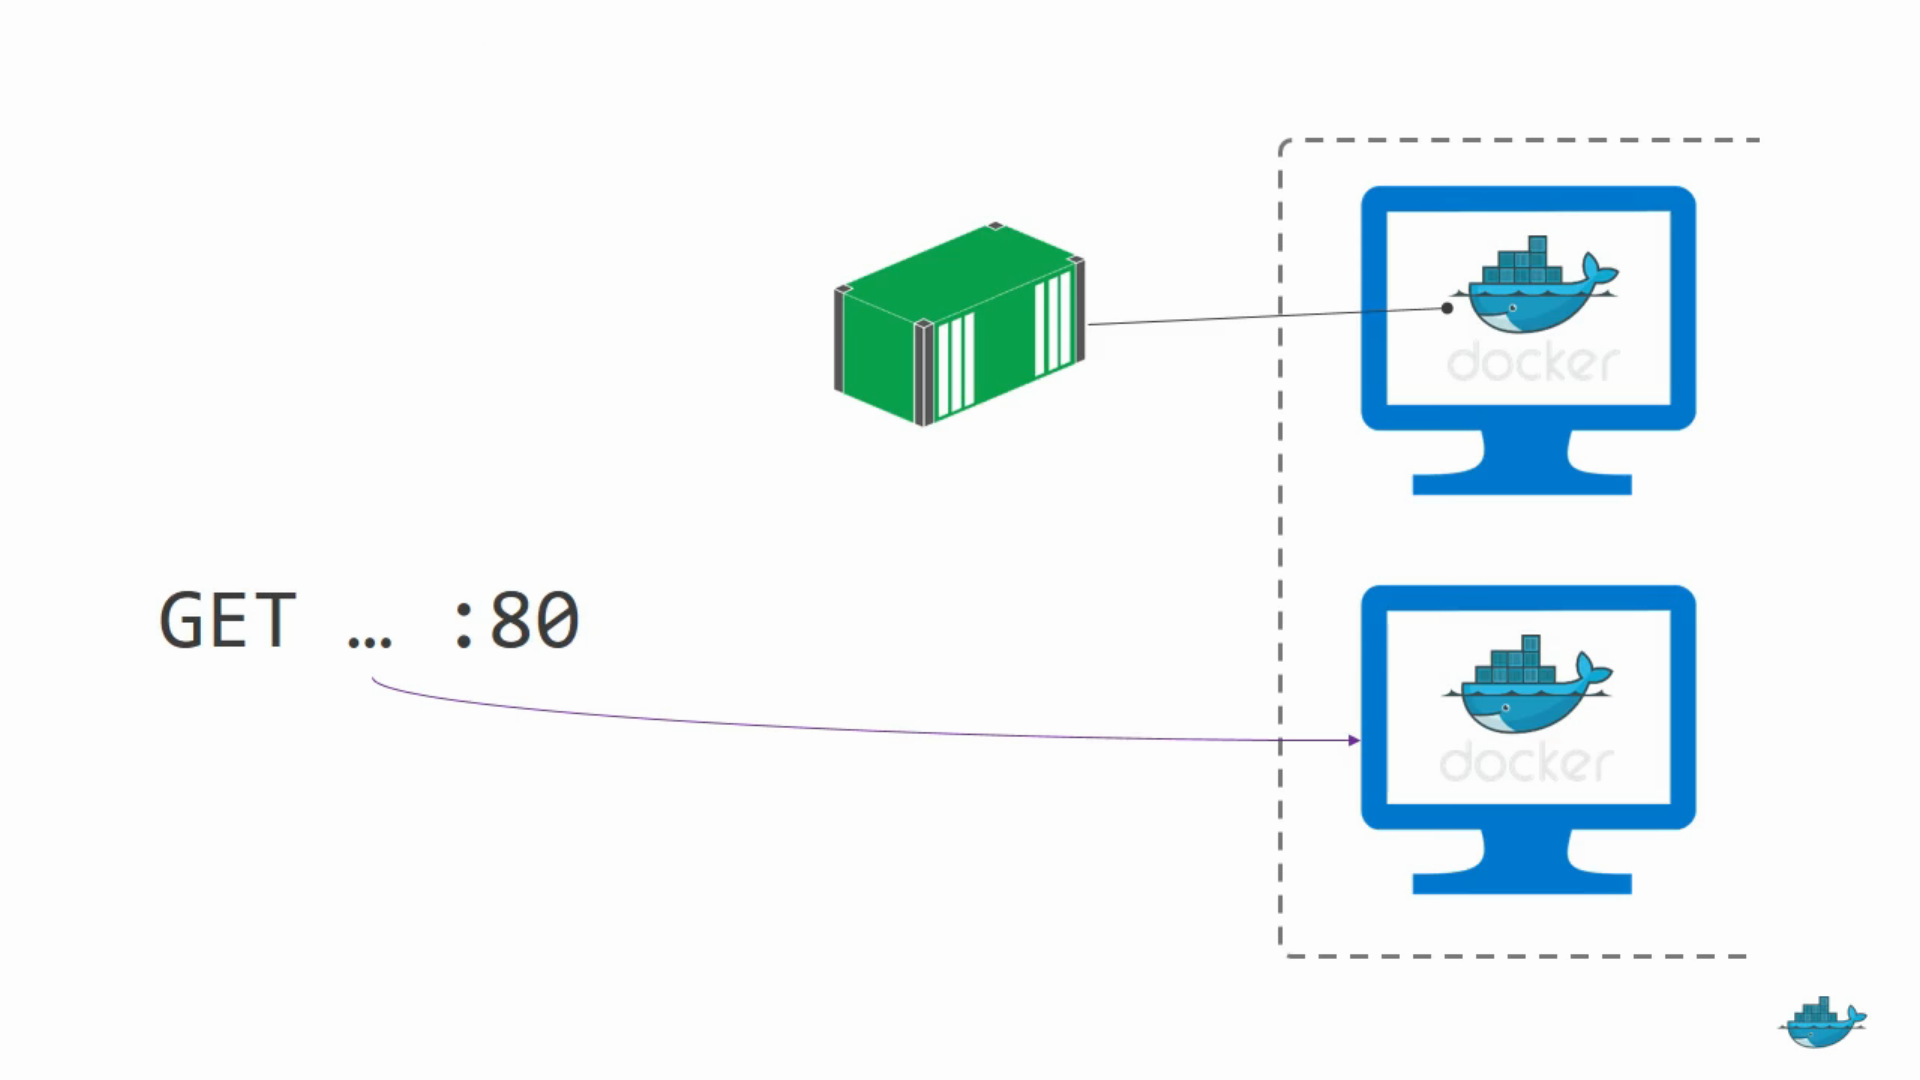
\includegraphics[width=0.95\linewidth]{img/orquestacion_11.png}
	\end{figure}
\end{frame}

\begin{frame}
  \frametitle{Algo sobre orquestación (12)}
	\begin{figure}[htp]
	\centering
	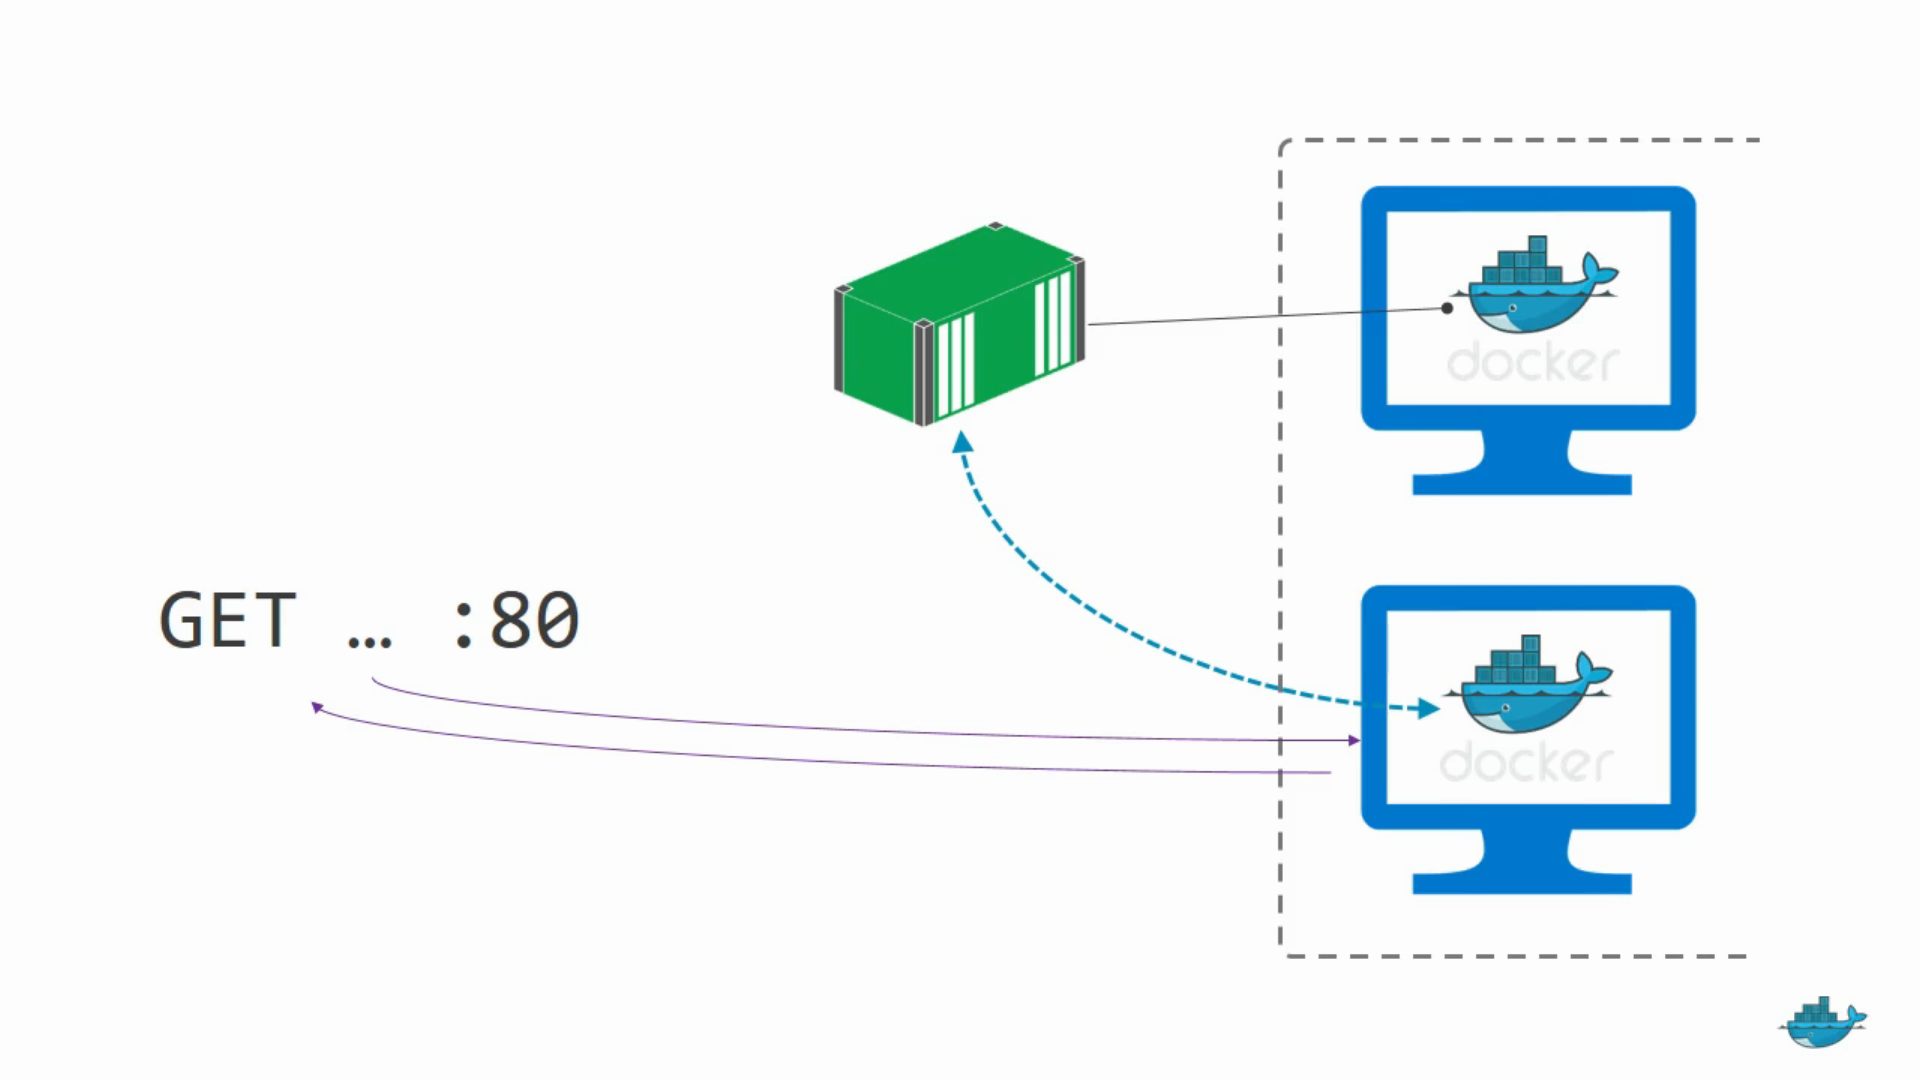
\includegraphics[width=0.95\linewidth]{img/orquestacion_12.png}
	\end{figure}
\end{frame}

\begin{frame}
  \frametitle{Algo sobre orquestación (13)}
	\begin{figure}[htp]
	\centering
	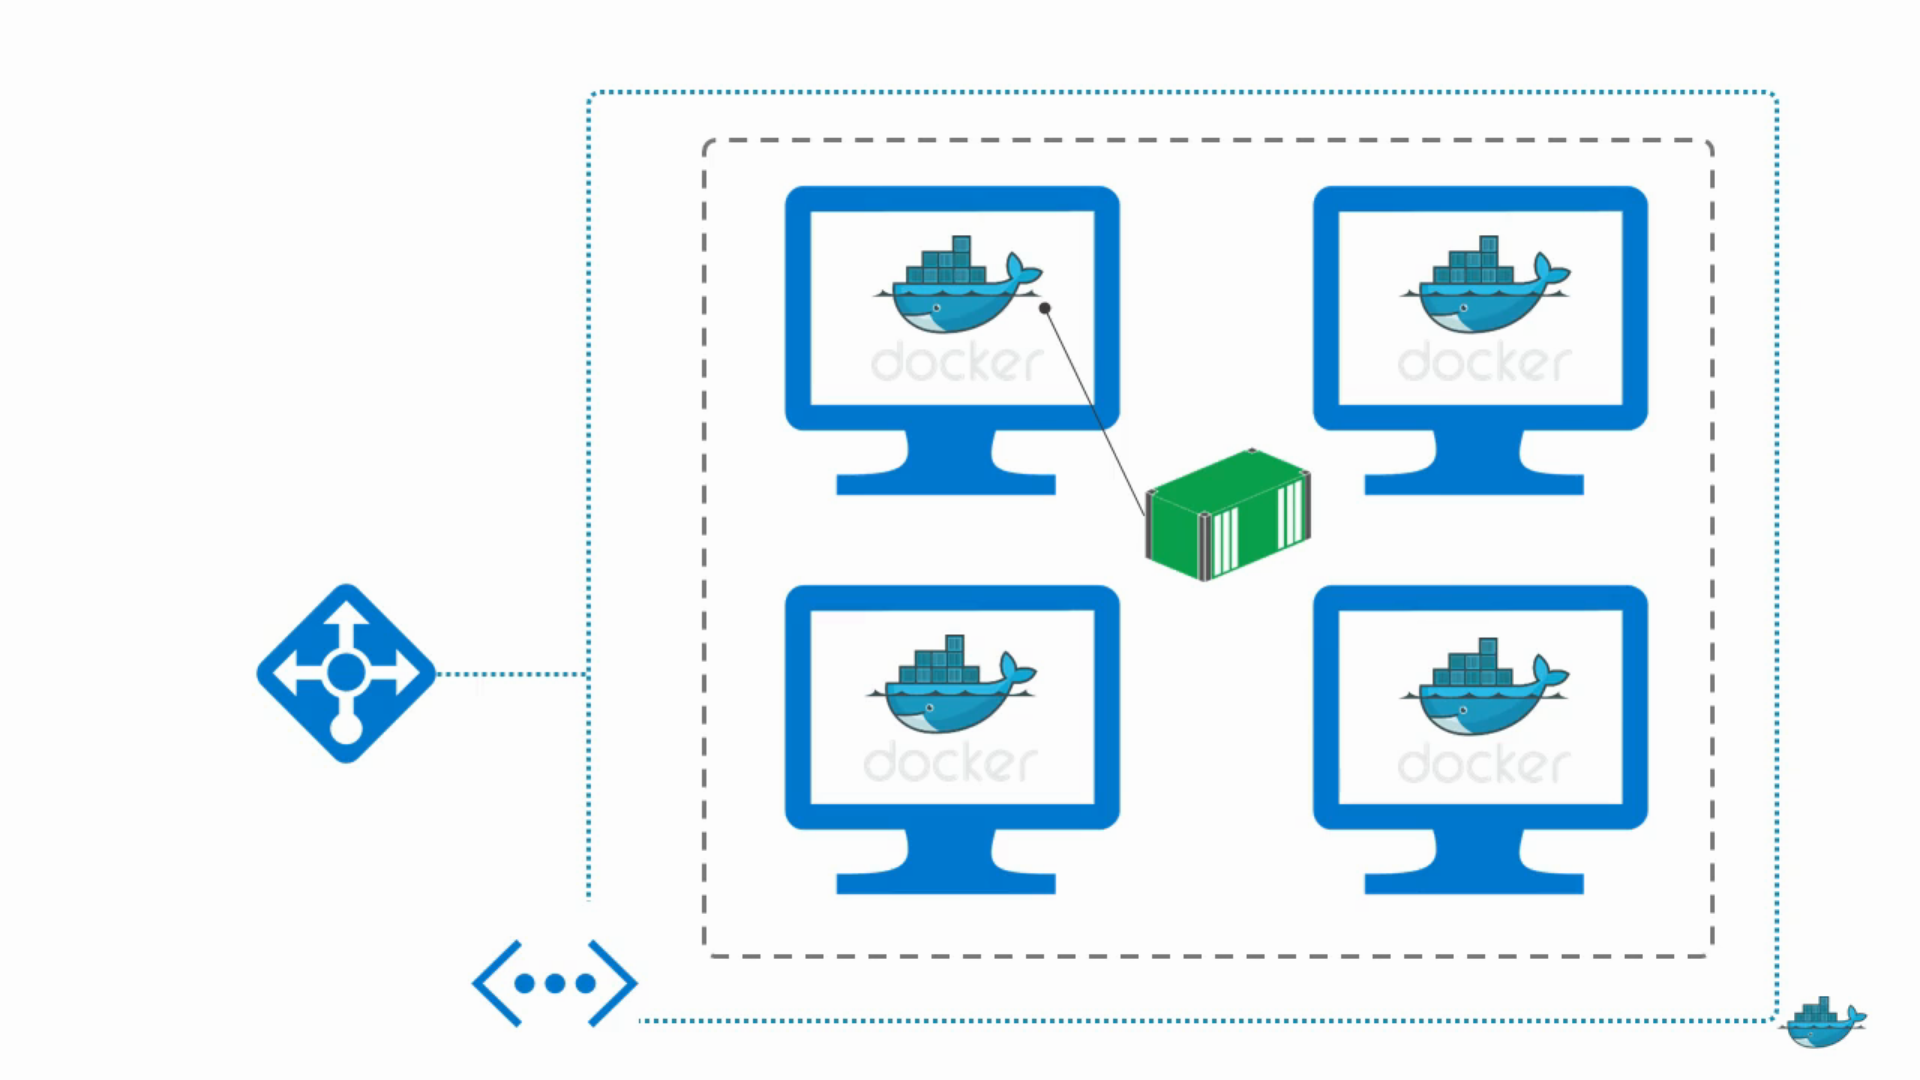
\includegraphics[width=0.95\linewidth]{img/orquestacion_13.png}
	\end{figure}
\end{frame}

\begin{frame}
  \frametitle{Algo sobre orquestación (14)}
	\begin{figure}[htp]
	\centering
	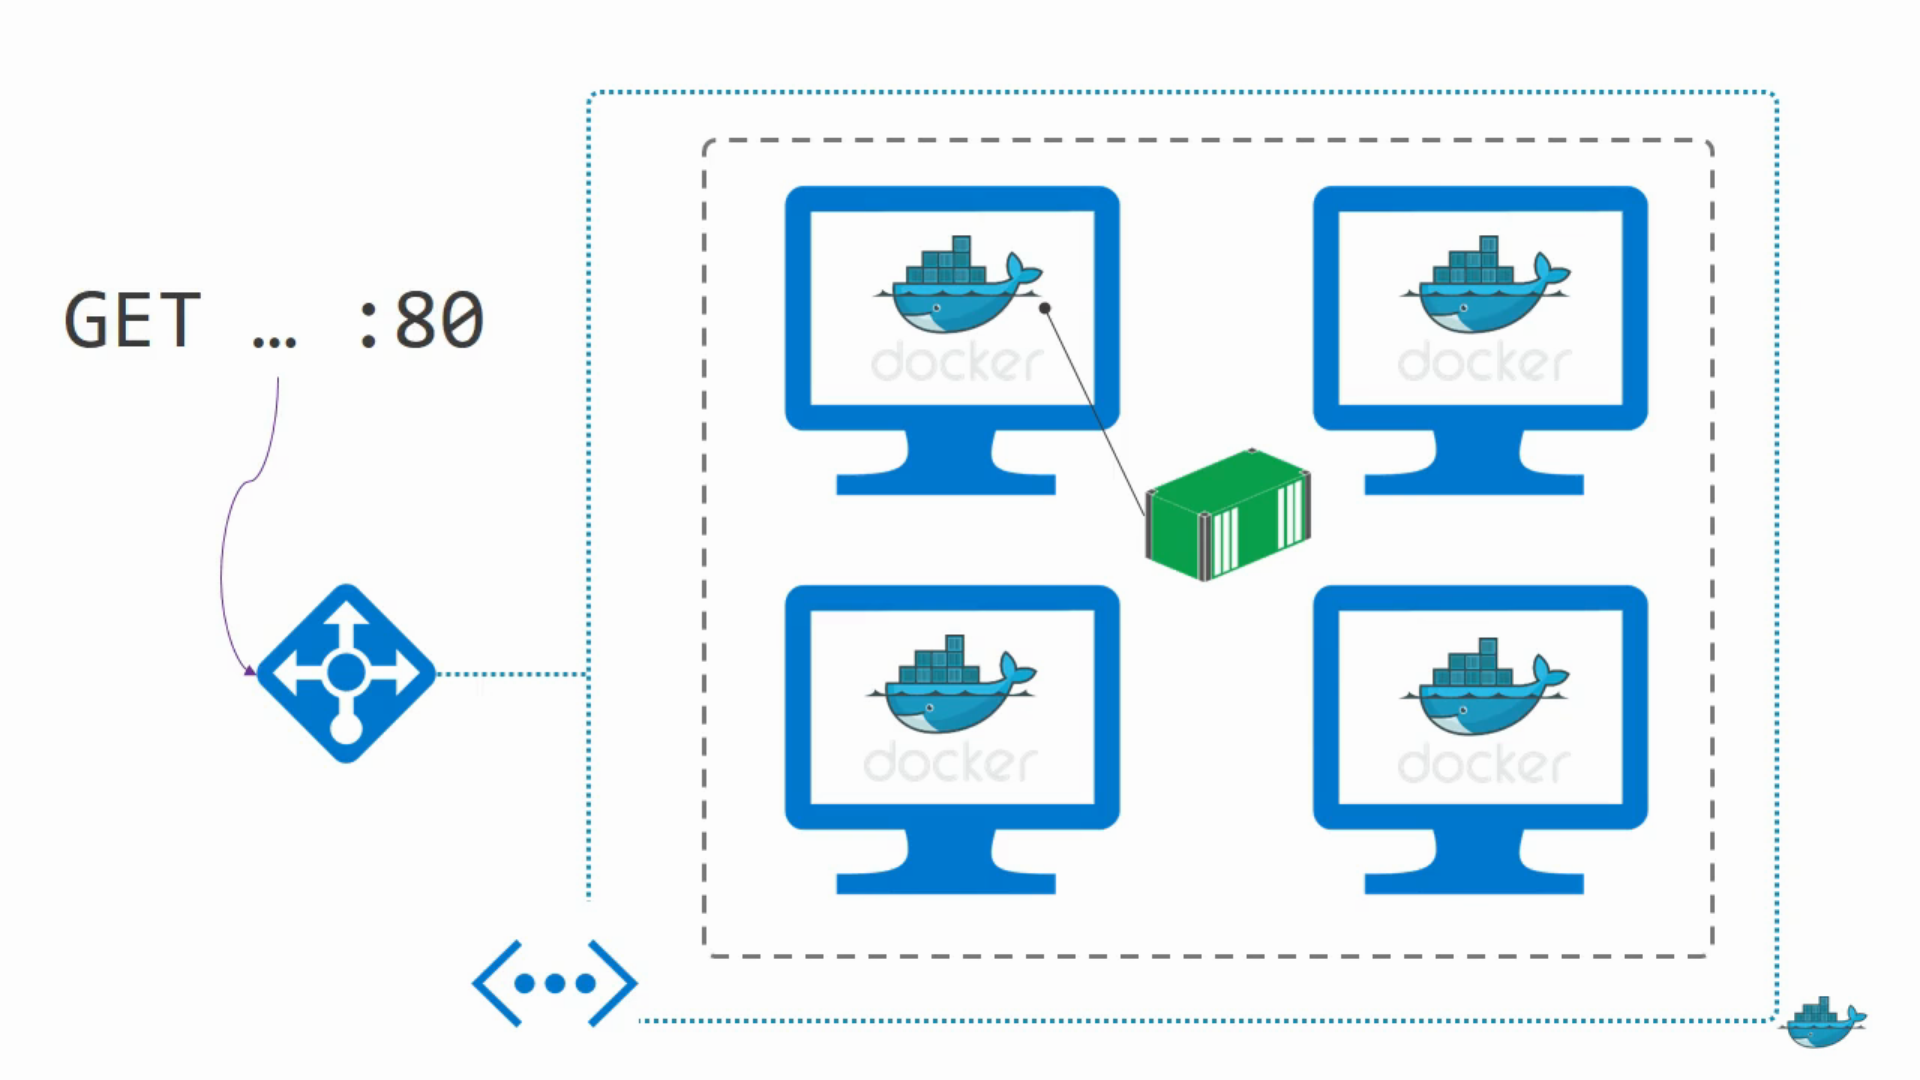
\includegraphics[width=0.95\linewidth]{img/orquestacion_14.png}
	\end{figure}
\end{frame}

\section{Qué vamos a hacer?}

\begin{frame}
  	\frametitle{Paso a paso}
	\begin{figure}[htp]
	\centering
	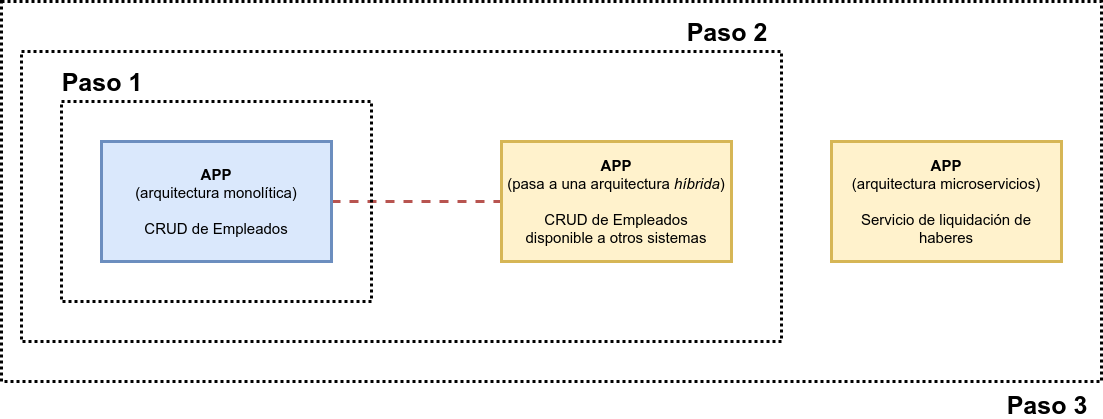
\includegraphics[width=0.95\linewidth]{img/paso-a-paso.png}
	\end{figure}
\end{frame}

\section{Ejemplos}

\begin{frame}
  	\frametitle{Demo}
  	
\end{frame}

\section{Cierre}

\begin{frame}
	\frametitle{Cuestiones a considerar antes de pasarse a microservicios}
	\begin{enumerate}
		\list Cómo se va a probar?
		\list Cómo se va a configurar?
		\list Cómo lo van a consumir otros servicios?
		\list Cómo se va a manejar la seguridad?
		\list Cómo se va a manejar el descubrimiento de servicios?
		\list Cómo va a escalar?
		\list Cómo se van a manejar los fallos?
		\list Cómo se van a manejar los cambios?
		\list Cómo se va a monitorear y medir el rendimiento?
	\end{enumerate}
\end{frame}

\begin{frame}
    \frametitle{Preguntas?}

\end{frame}

\begin{frame}
    \frametitle{Gracias}
	Contactos:\\
    \begin{itemize}
	\item {Martín Rey: martinrey@fceqyn.unam.edu.ar}
	\item {Ulises Ramirez: ulisesramirez@fceqyn.unam.edu.ar}
	\end{itemize}

	Instituto de Desarrollo, Innovación e Investigación en Informática \\ FCEQyN - UNaM
\end{frame}

\end{document}
